\documentclass[a4paper,12pt]{article}
\usepackage[utf8]{vietnam}
\usepackage{hyperref}
\usepackage{graphicx}
\usepackage{xcolor}
\usepackage{subfigure}
\usepackage{float}
\usepackage{caption}
\hypersetup{
	pdfborder = {0 0 0}
}
\title{\textbf{Báo cáo tuần 3 \\ Thực hành kiến trúc máy tính}}
\author{Họ tên: Phan Minh Anh Tuấn \\ MSSV: 20205227}
\date{}
\begin{document}
\maketitle
\tableofcontents
\newpage
%\section{Home Assignment 1}
%\begin{figure}[!h]
%	\centering
%	\subfigure{ 
%		\includegraphics[scale = 0.3]{flowchart.png}
%		\label{flowchart}} 
%	\subfigure{ 
%		\includegraphics[scale = 0.515]{home1.png}
%		\label{Code}}  
%	\caption{Lưu đồ và code của bài toán} 
%\end{figure}
%\clearpage
%\newpage
%\section{Home Assignment 2}
%
%\section{Home Assignment 3}
\section{Assignment 1}
Mã số sinh viên của em: 20205227, mã số sinh viên bạn ngồi cạnh: 20205231 \\
Đặt i = 5227, j = 5231 \\
\begin{figure}[!h]
	\centerline{\fbox{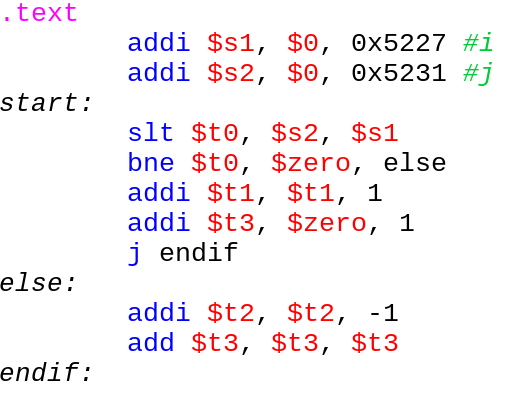
\includegraphics[width=0.7\textwidth]{ass1/ass1.png}}}
	\caption{Code của Assignment 1}
	\label{fig:ass1}
\end{figure}
\begin{figure}[!h]
	\centerline{\fbox{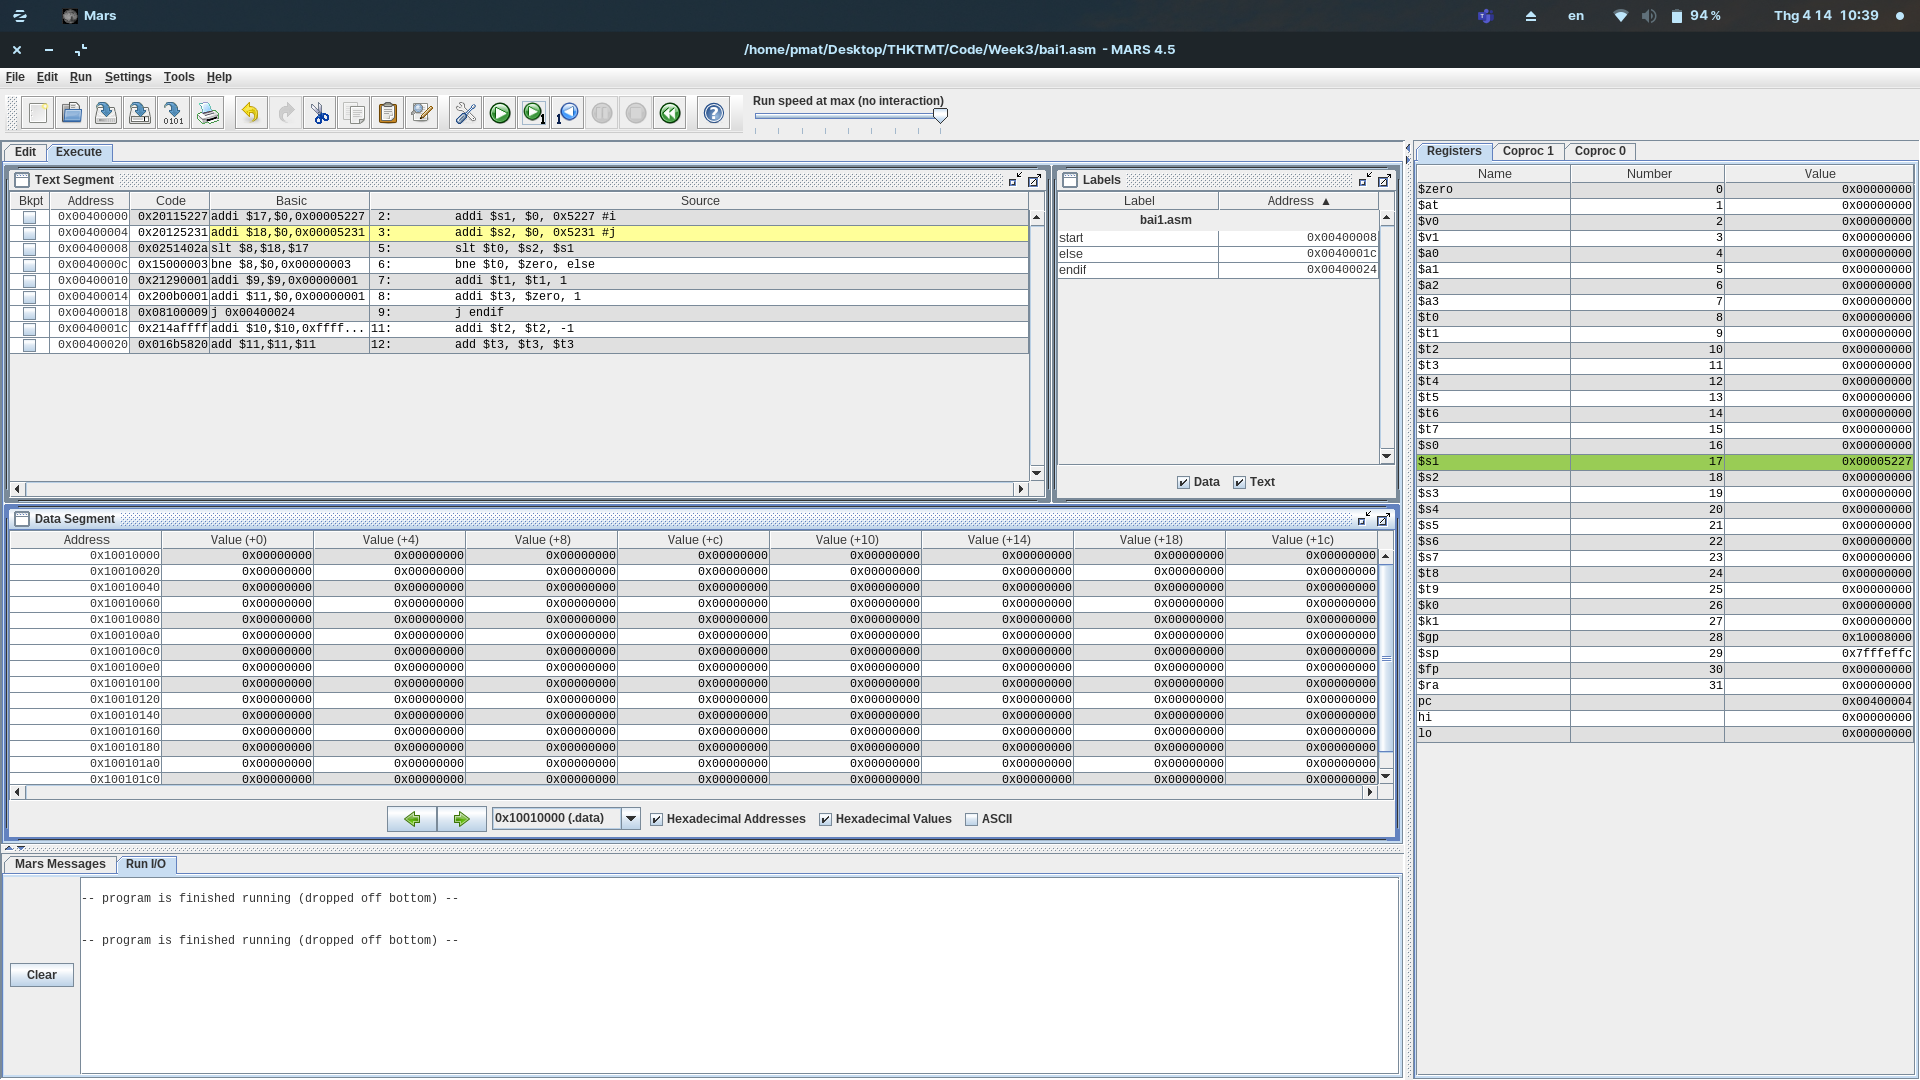
\includegraphics[width=0.7\textwidth]{ass1/s1.png}}}
	\caption*{Step 1: Gán thanh ghi \$s1 (i) giá trị 5227}
	\label{fig:s1}
\end{figure}
\begin{figure}[!h]
	\centerline{\fbox{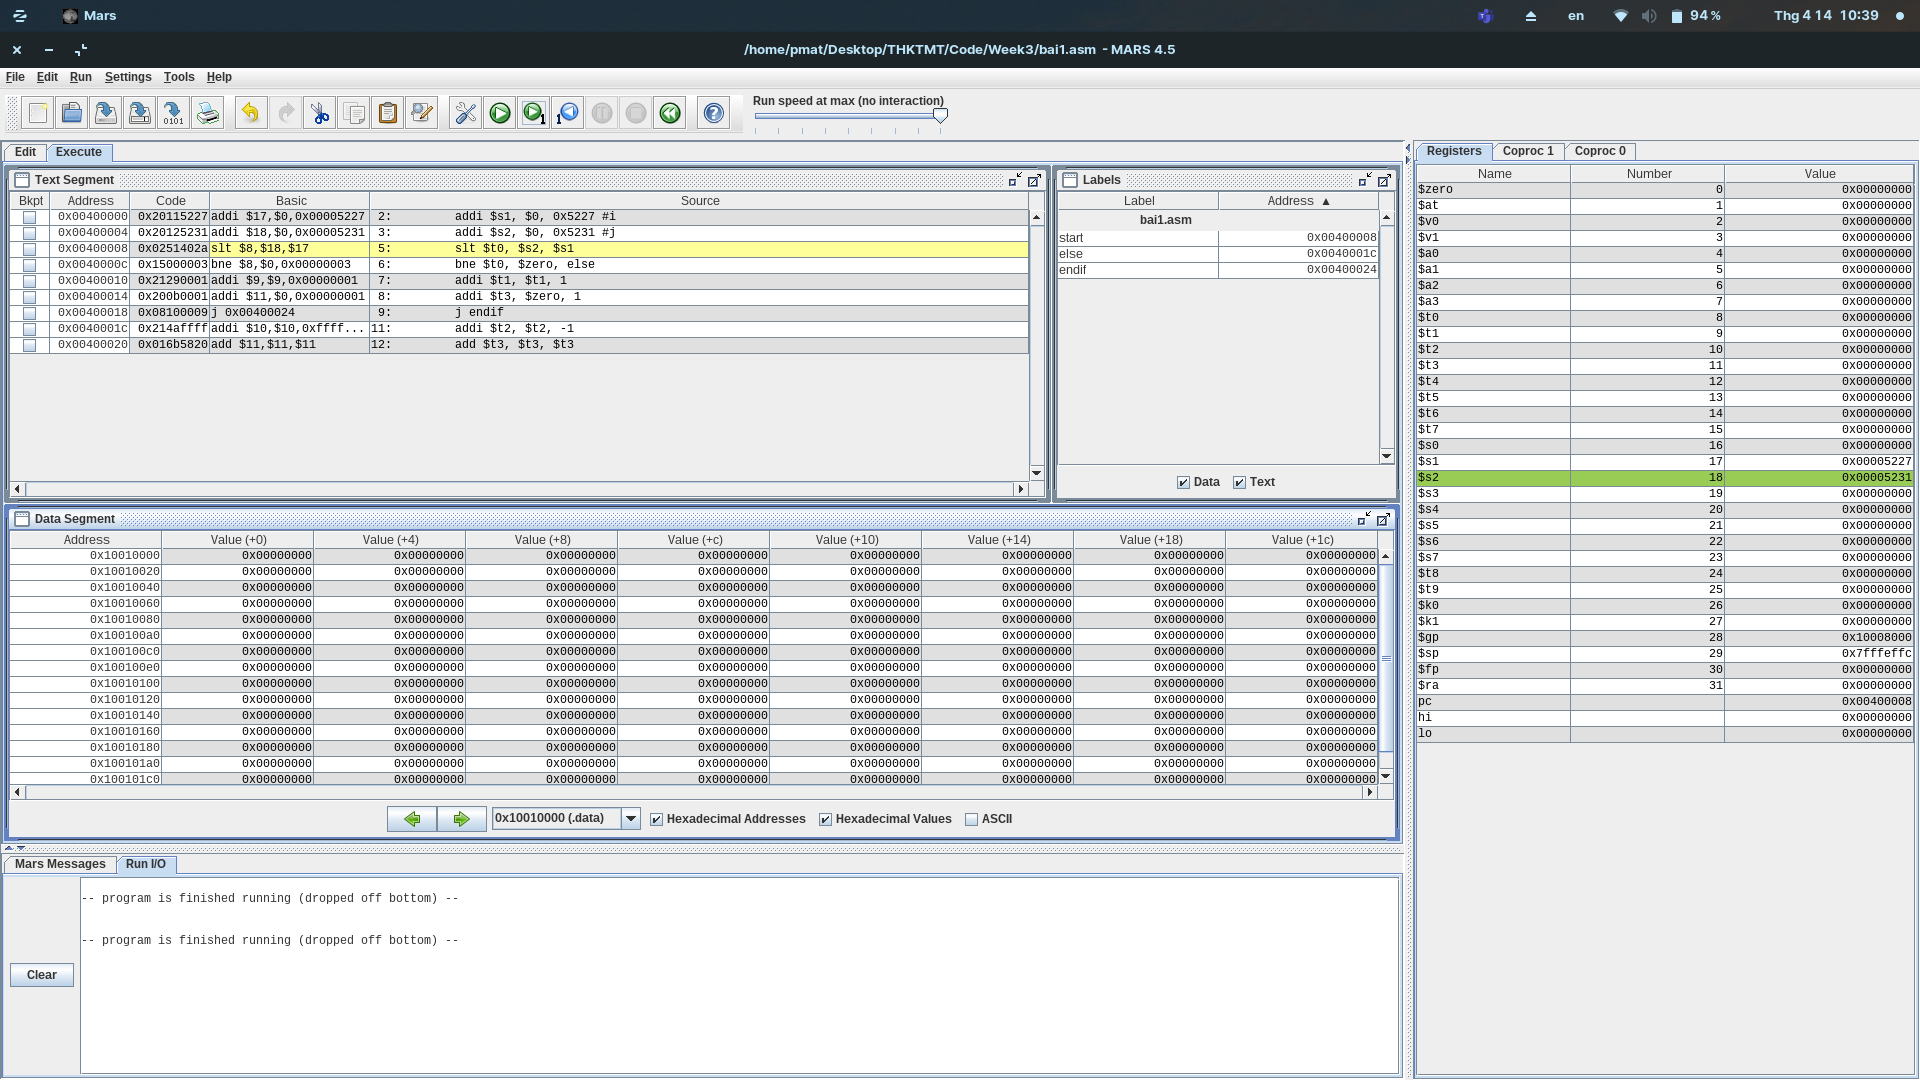
\includegraphics[width=0.7\textwidth]{ass1/s2.png}}}
	\caption*{Step 2: Gán thanh ghi \$s2 (j) giá trị 5231}
	\label{fig:s2}
\end{figure}
\begin{figure}[!h]
	\centerline{\fbox{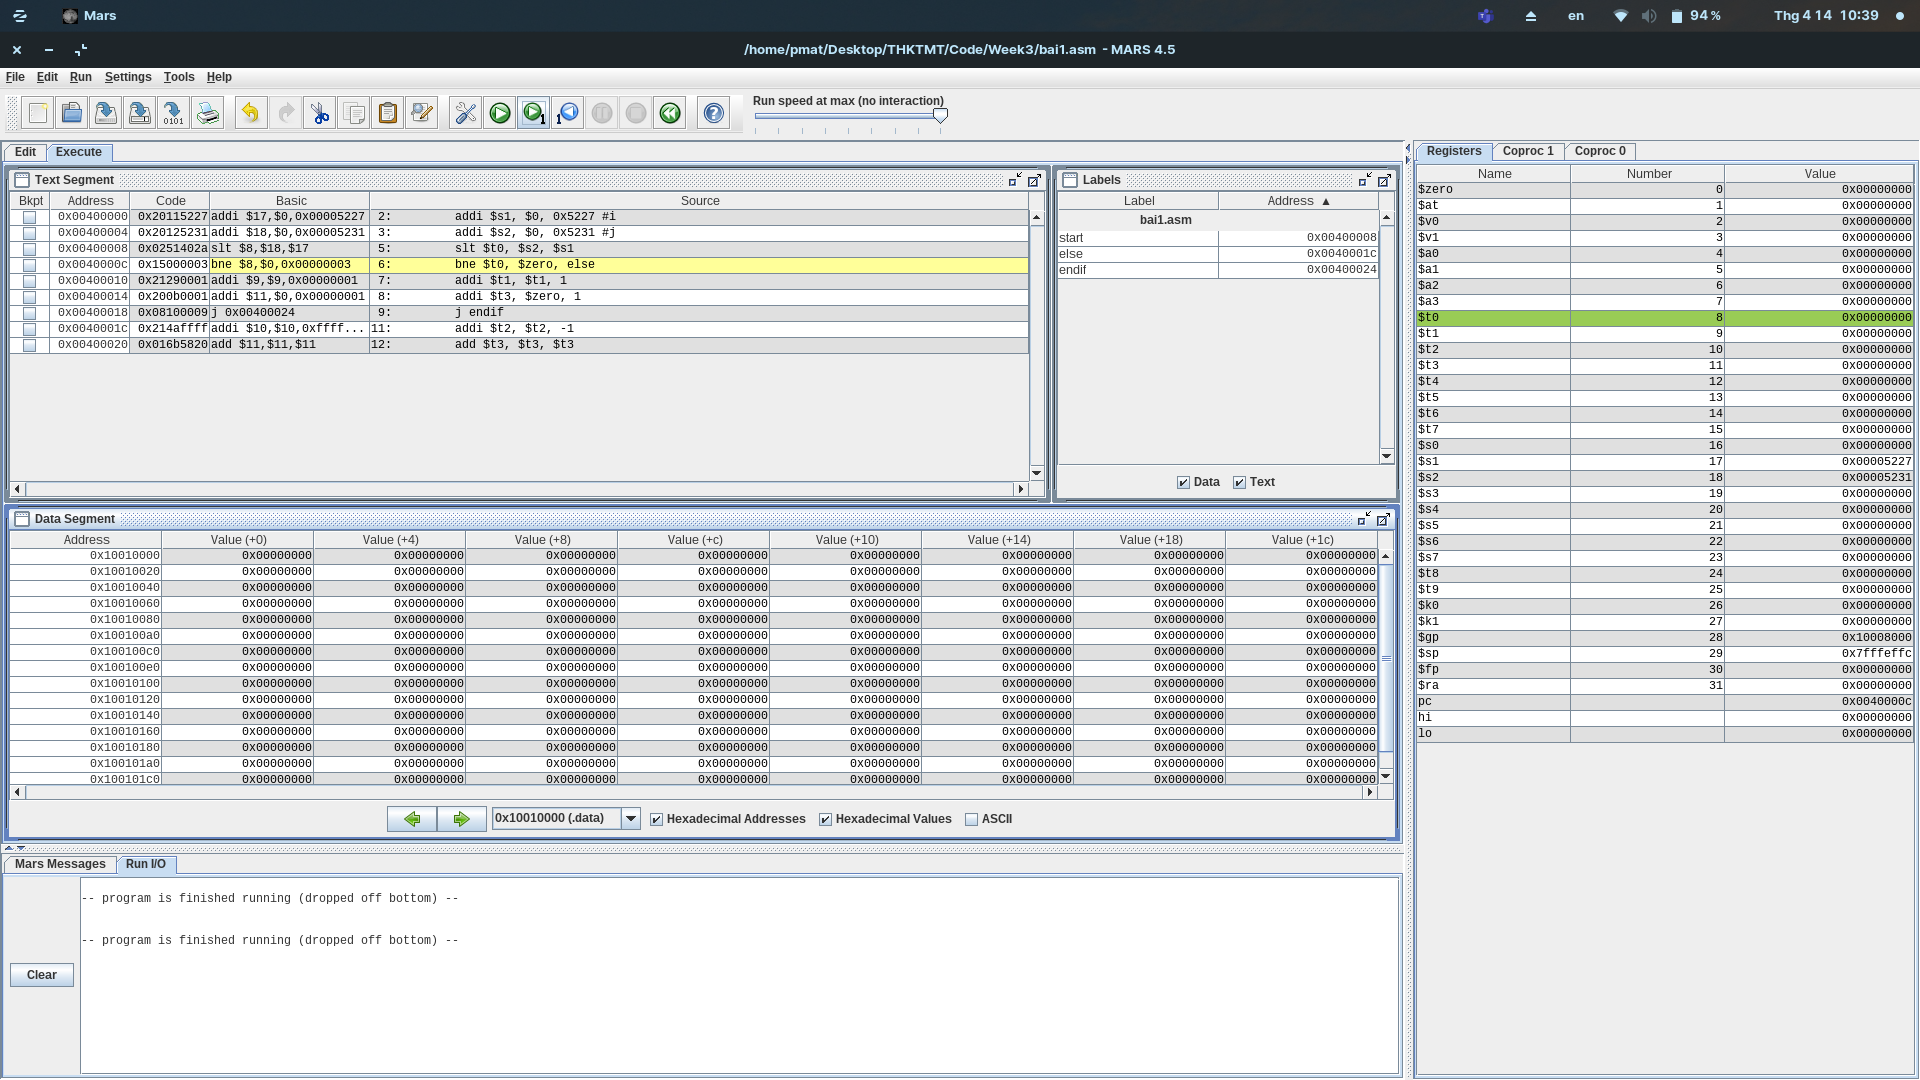
\includegraphics[width=0.7\textwidth]{ass1/s3.png}}}
	\caption*{Step 3: So sánh j và j, \$t0 = 0 do \$s2 > \$s1}
	\label{fig:s3}
\end{figure}
\begin{figure}[!h]
	\centerline{\fbox{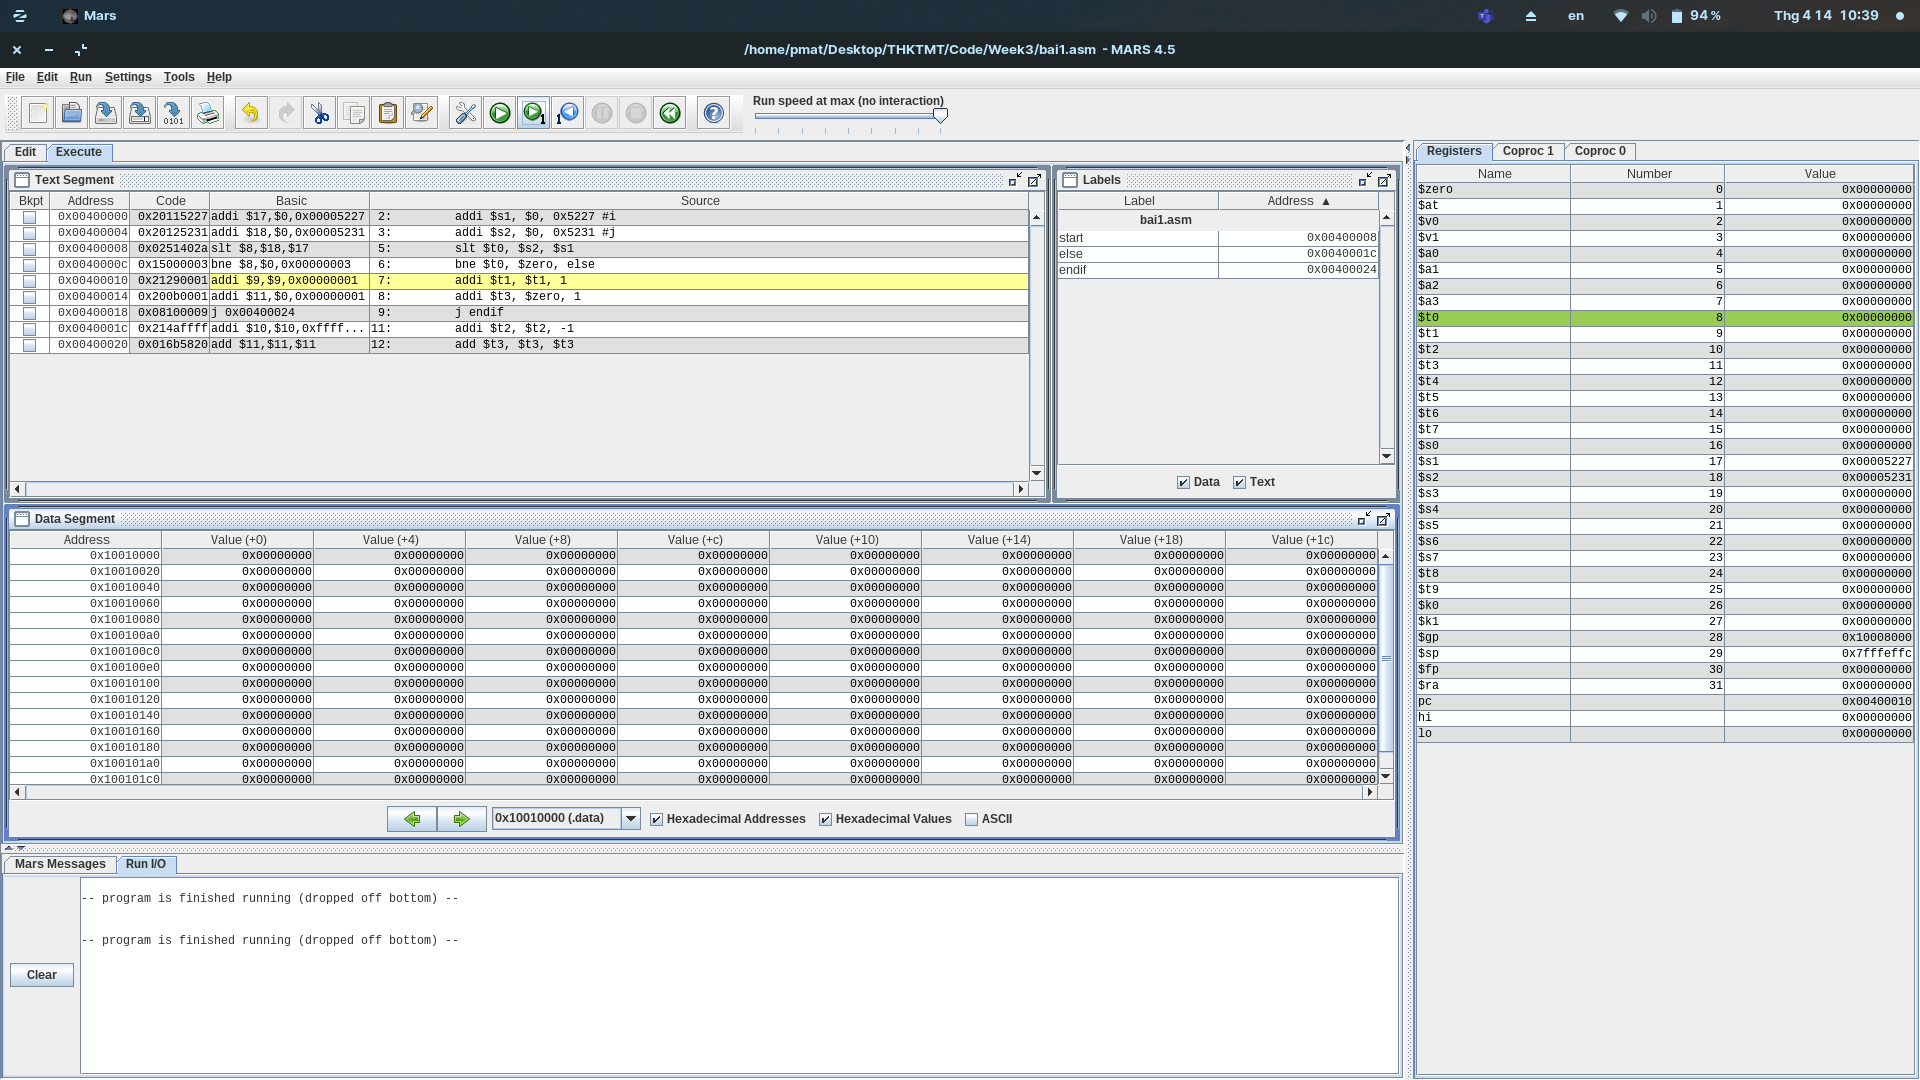
\includegraphics[width=0.7\textwidth]{ass1/s4.png}}}
	\caption*{Step 4: So sánh \$t0 với 0, nếu \$t0 != 0 nhảy đến else}
	\label{fig:s4}
\end{figure}
\begin{figure}[!h]
	\centerline{\fbox{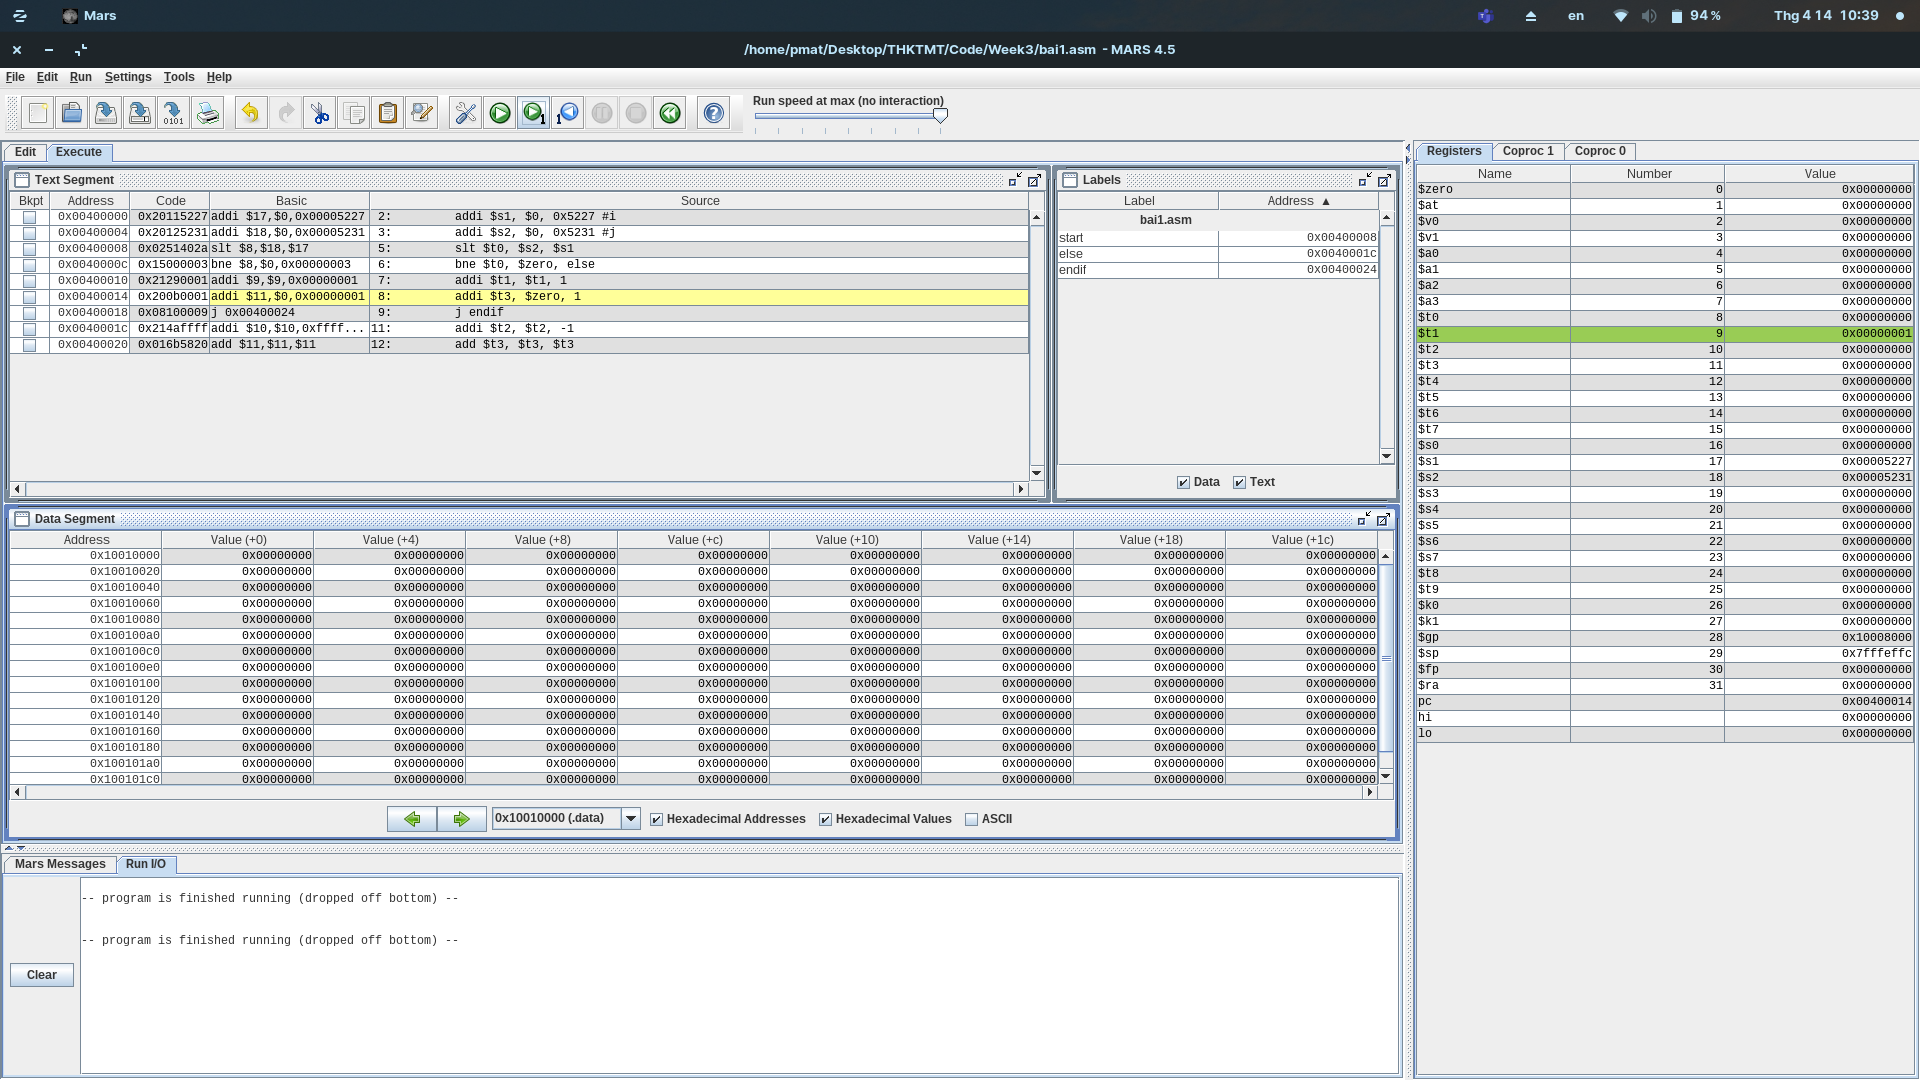
\includegraphics[width=0.7\textwidth]{ass1/s5.png}}}
	\caption*{Step 5: Do \$t0 == 0, thực hiện câu lệnh dưới: \$t1 = \$t1 + 1 = 0x1}
	\label{fig:s5}
\end{figure}
\begin{figure}[!h]
	\centerline{\fbox{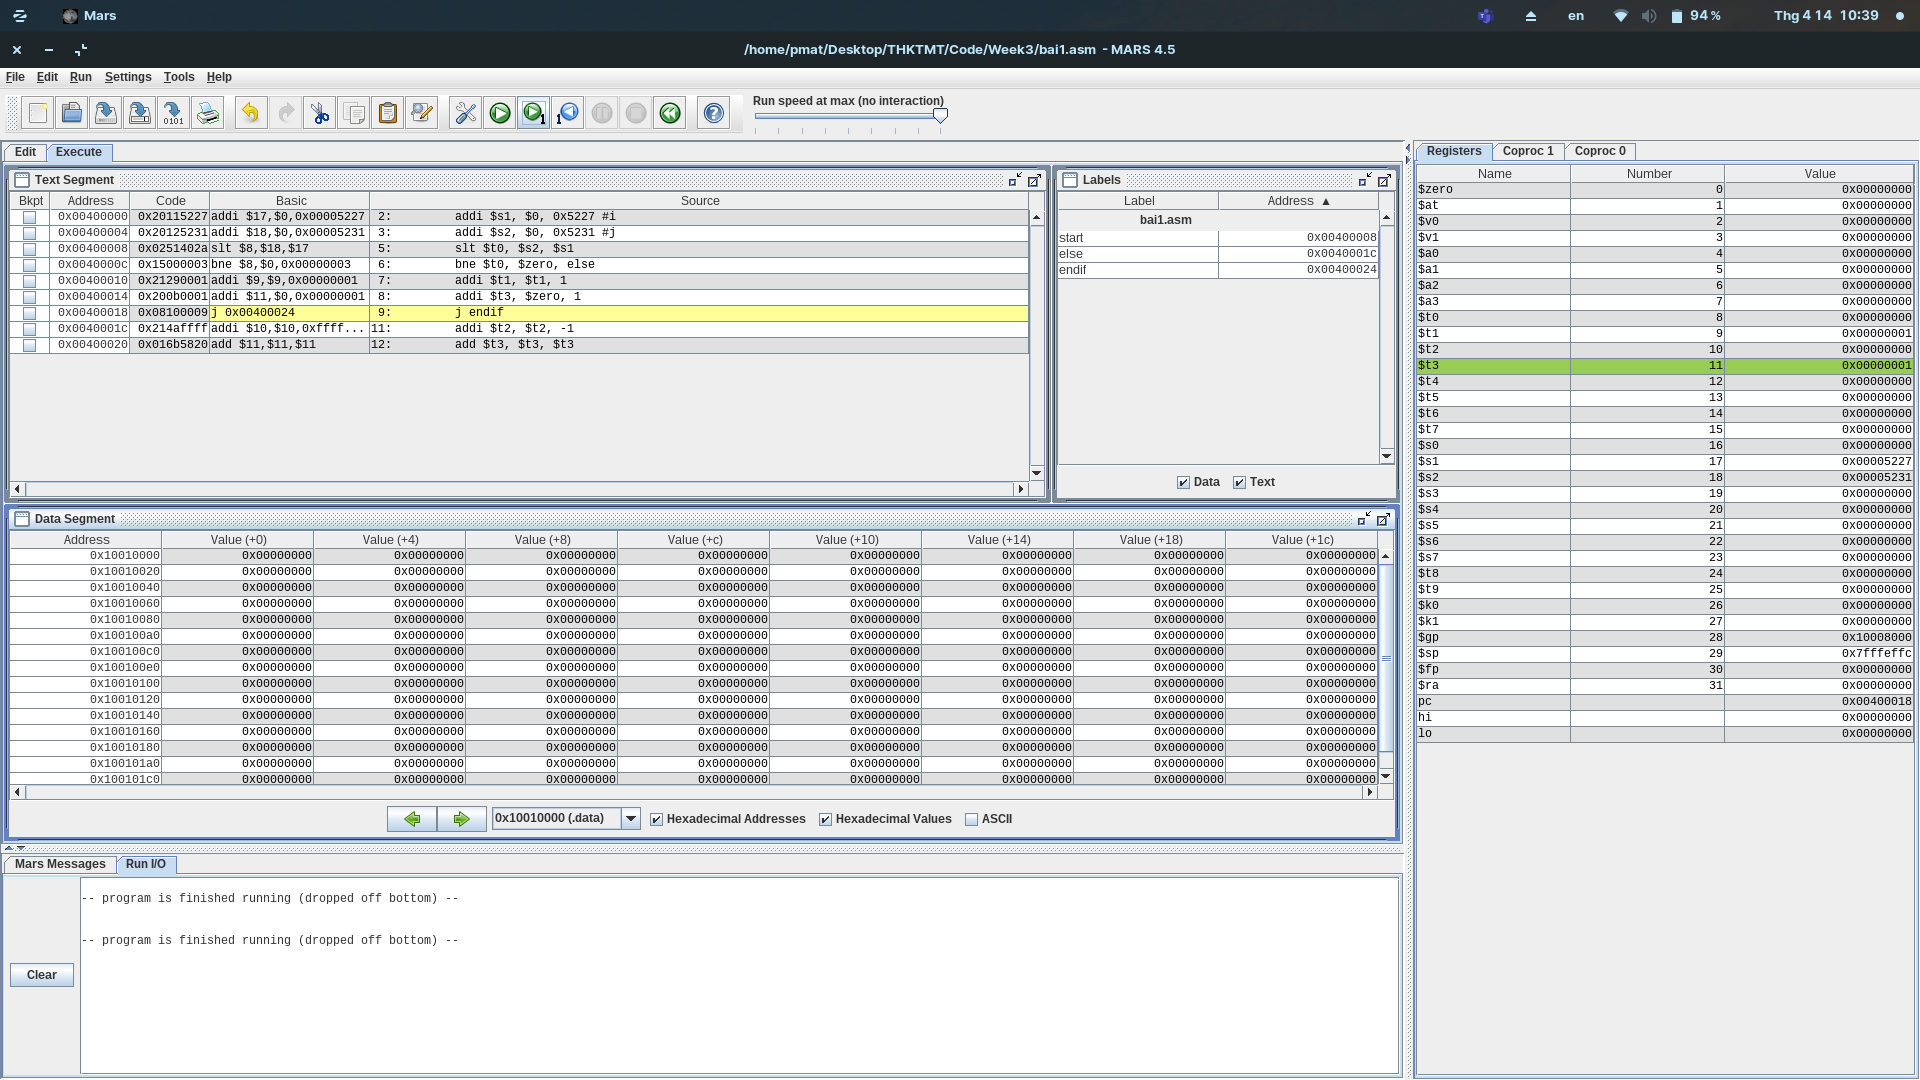
\includegraphics[width=0.7\textwidth]{ass1/s6.png}}}
	\caption*{Step 6: \$t3 = \$0 + 1 = 0x1}
	\label{fig:s6}
\end{figure}
\begin{figure}[!h]
	\centerline{\fbox{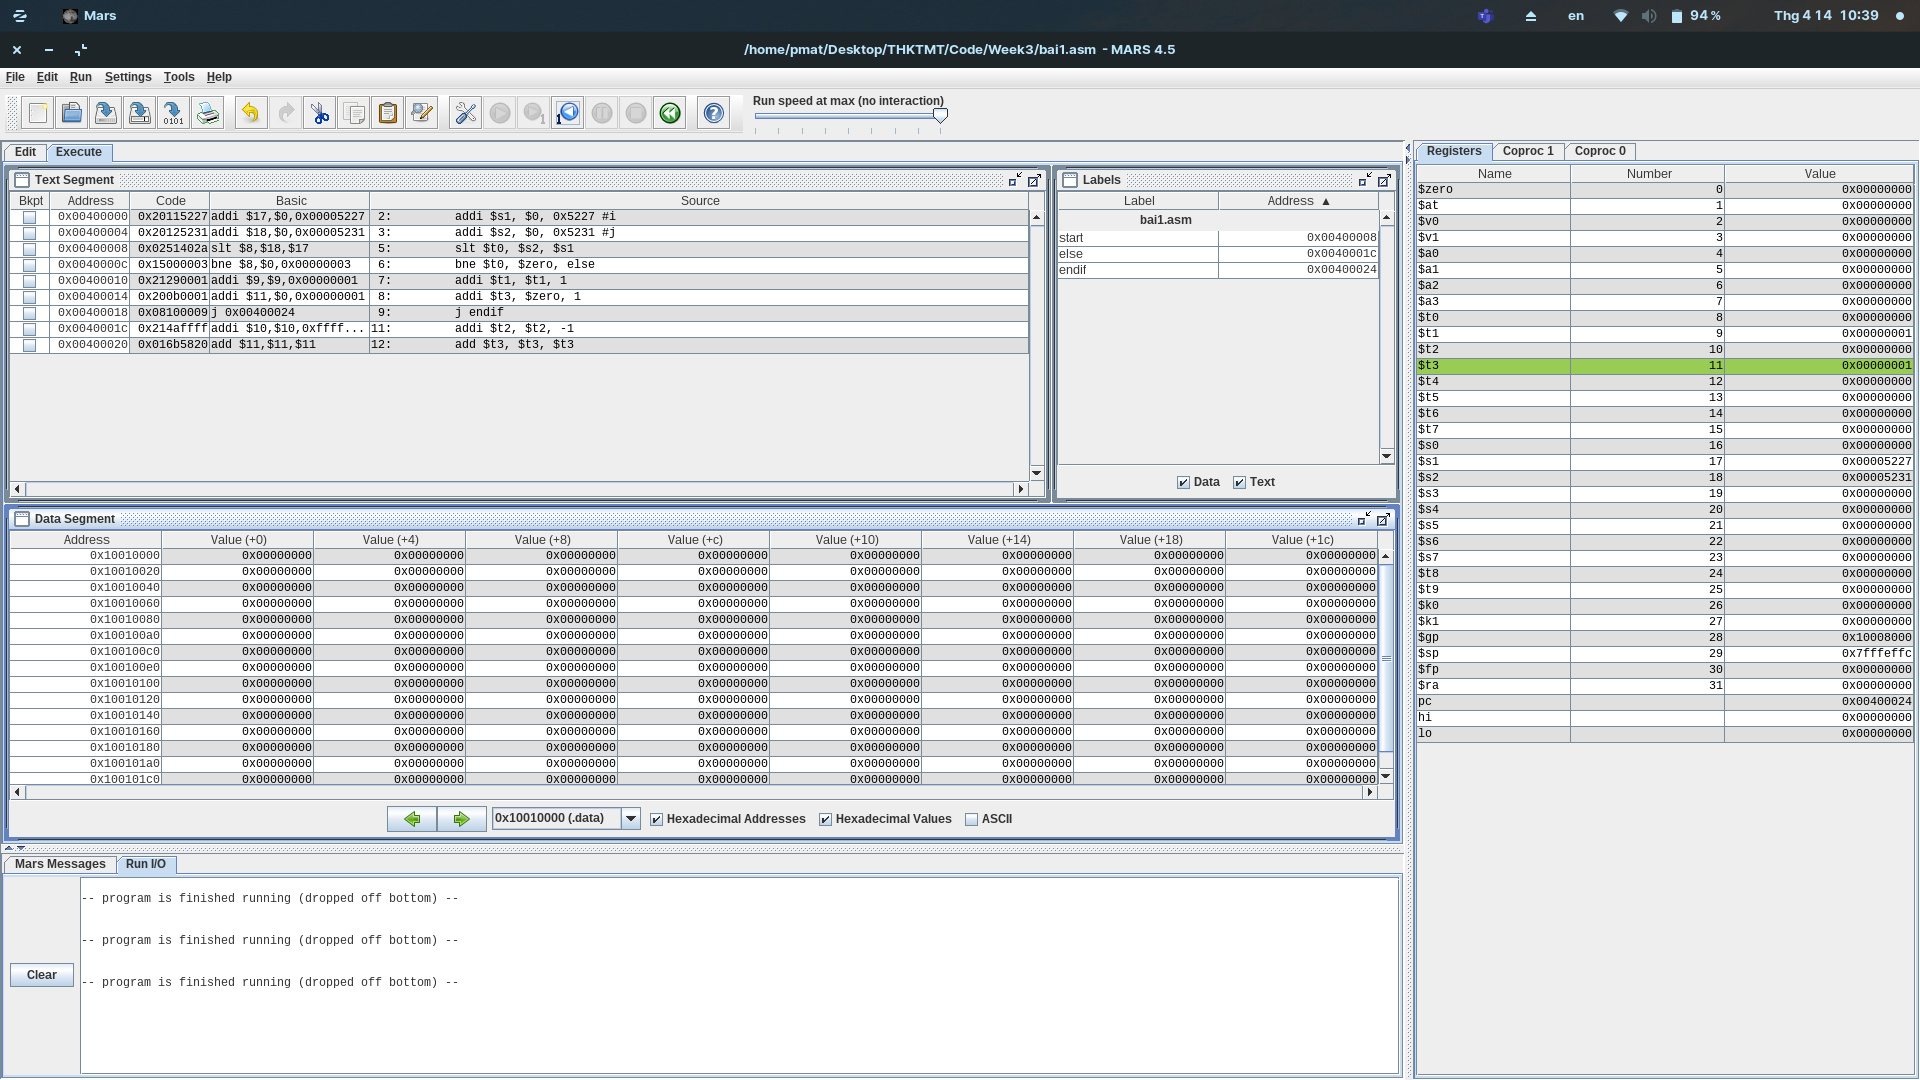
\includegraphics[width=0.7\textwidth]{ass1/s7.png}}}
	\caption*{Step 7: Nhảy đến endif, kết thúc chương trình}
	\label{fig:s7}
\end{figure}
\clearpage
\newpage
\section{Assignment 2}
\begin{figure}[!h]
	\centerline{\fbox{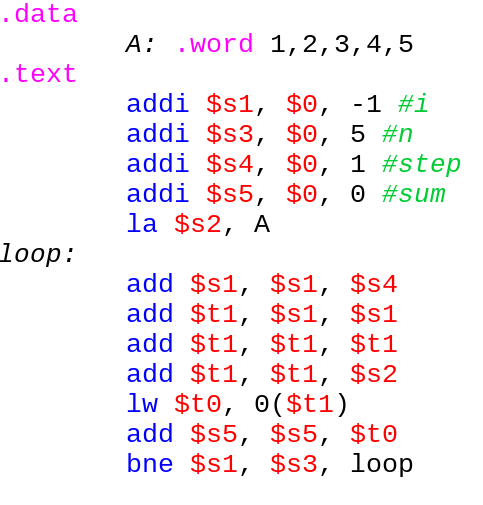
\includegraphics[width=0.7\textwidth]{ass2/ass2.png}}}
	\caption{Code của Assignment 2}
	\label{fig:ass2}
\end{figure}
\begin{figure}[!h]
	\centerline{\fbox{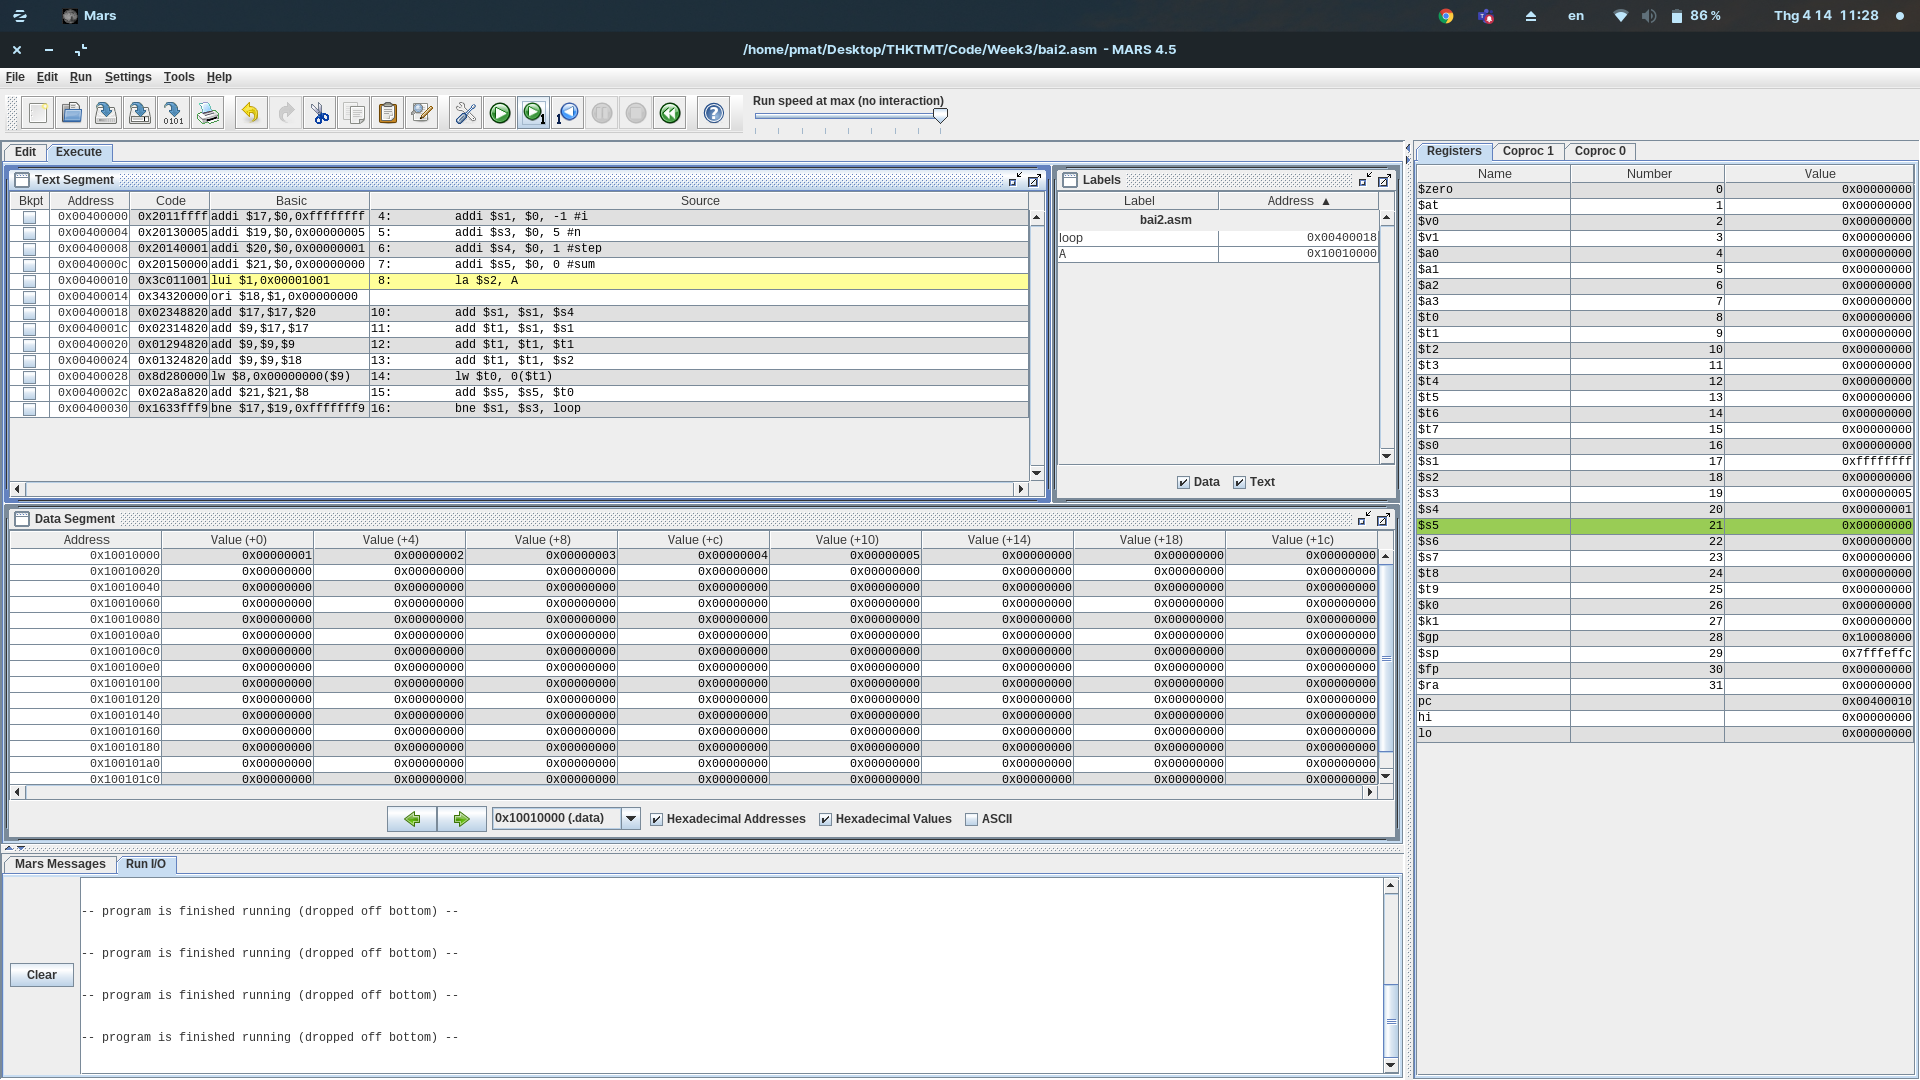
\includegraphics[width=0.7\textwidth]{ass2/s4.png}}}
	\caption*{Step 1: Gán giá trị thanh ghi lần lượt \$s1 = -1, \$s3 = 5, \$s4 = 1, \$s5 = 0}
	\label{fig:2s1}
\end{figure}
\begin{figure}[!h]
	\centerline{\fbox{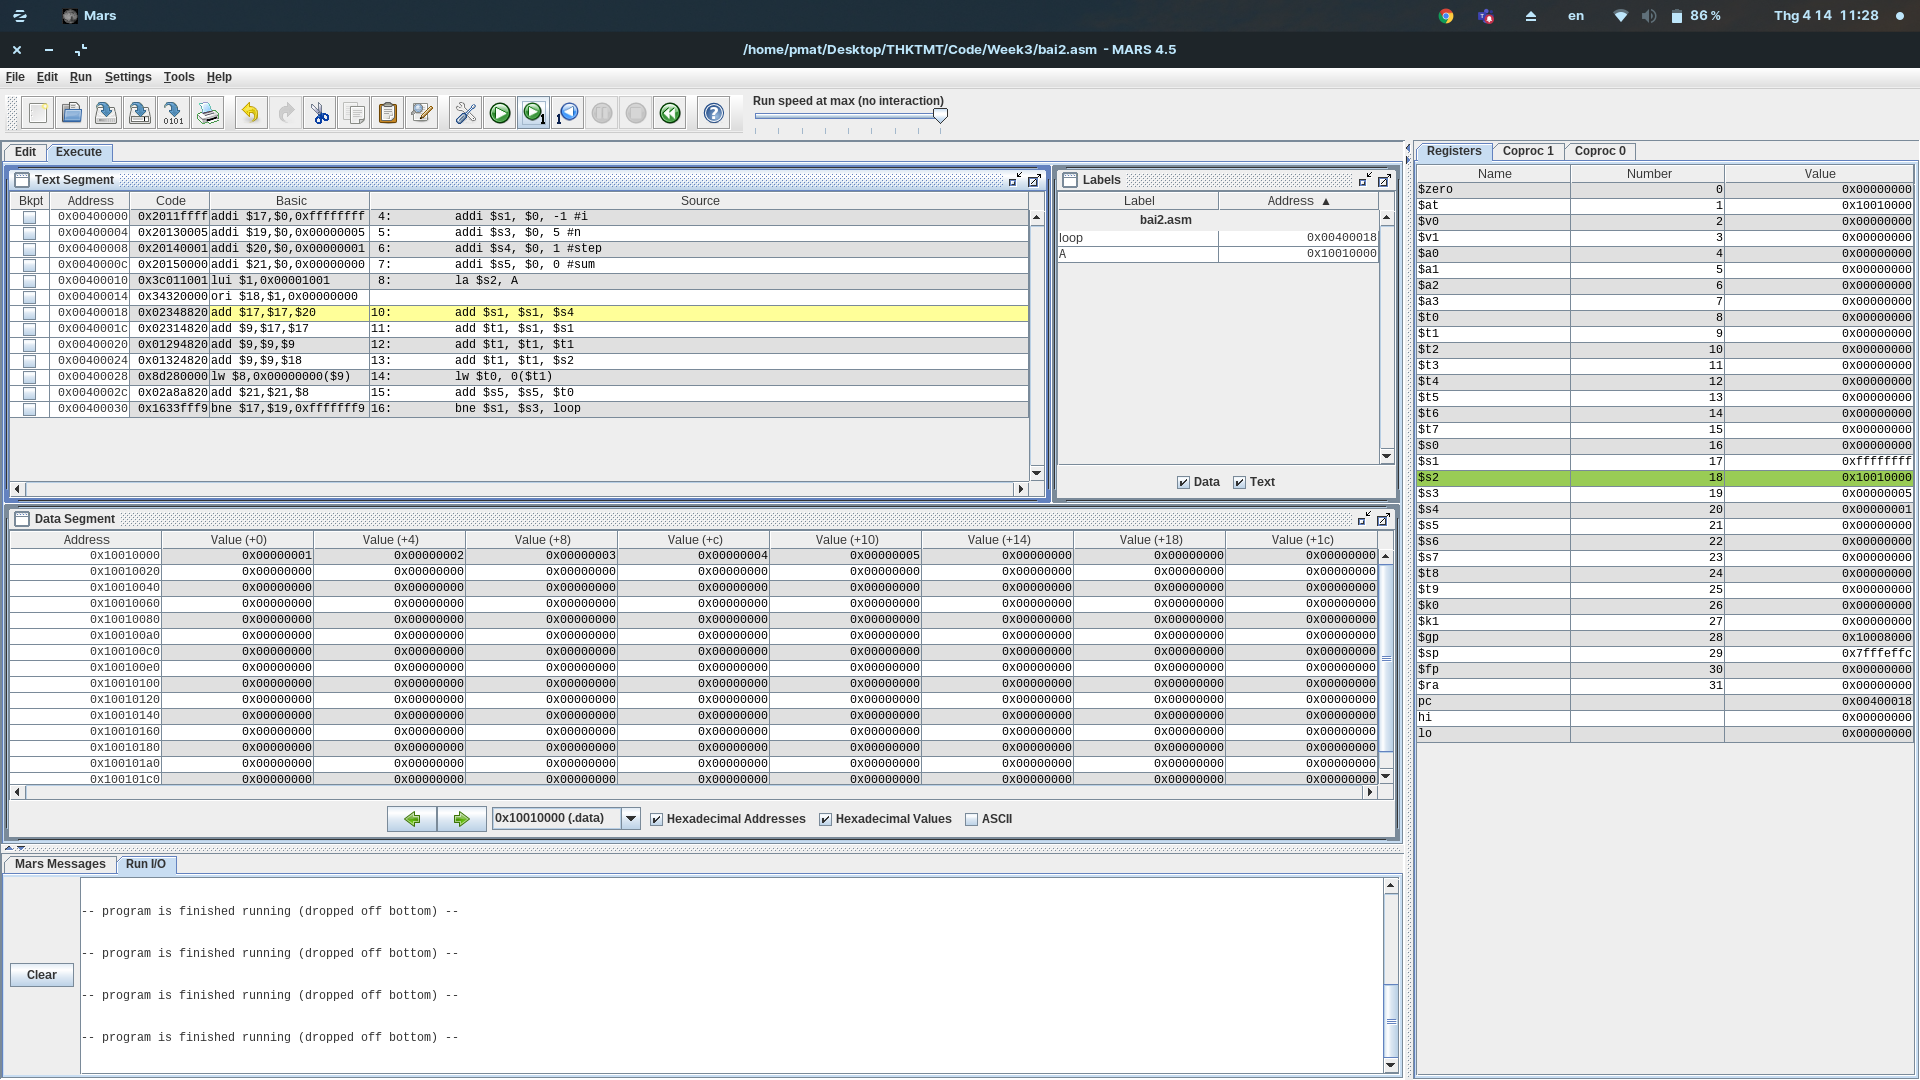
\includegraphics[width=0.7\textwidth]{ass2/s5.png}}}
	\caption*{Step 2: Load địa chỉ mảng A vào \$s2}
	\label{fig:2s2}
\end{figure}
\begin{figure}[!h]
	\centerline{\fbox{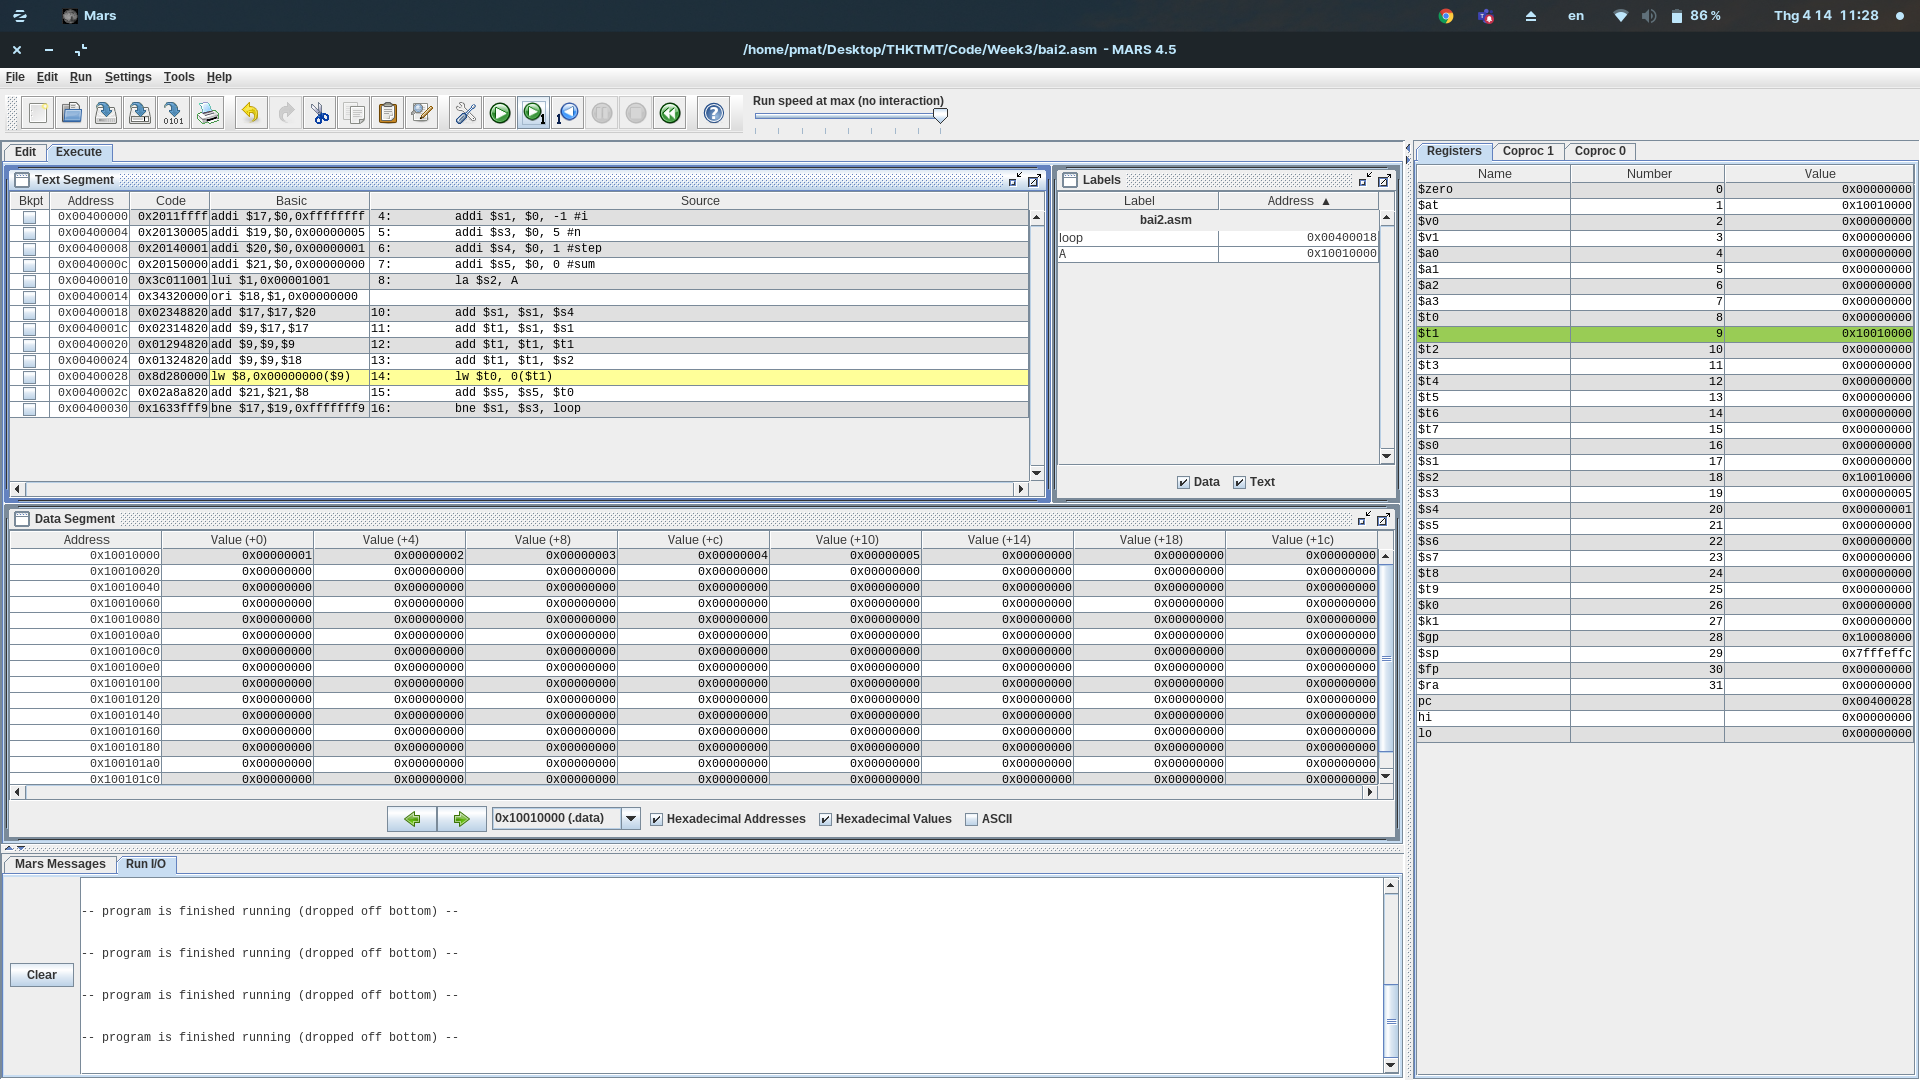
\includegraphics[width=0.7\textwidth]{ass2/s9.png}}}
	\caption*{Step 3: \$t1 lưu trữ địa chỉ trỏ đến phần tử hiện tại của mảng}
	\label{fig:2s3}
\end{figure}
\begin{figure}[!h]
	\centerline{\fbox{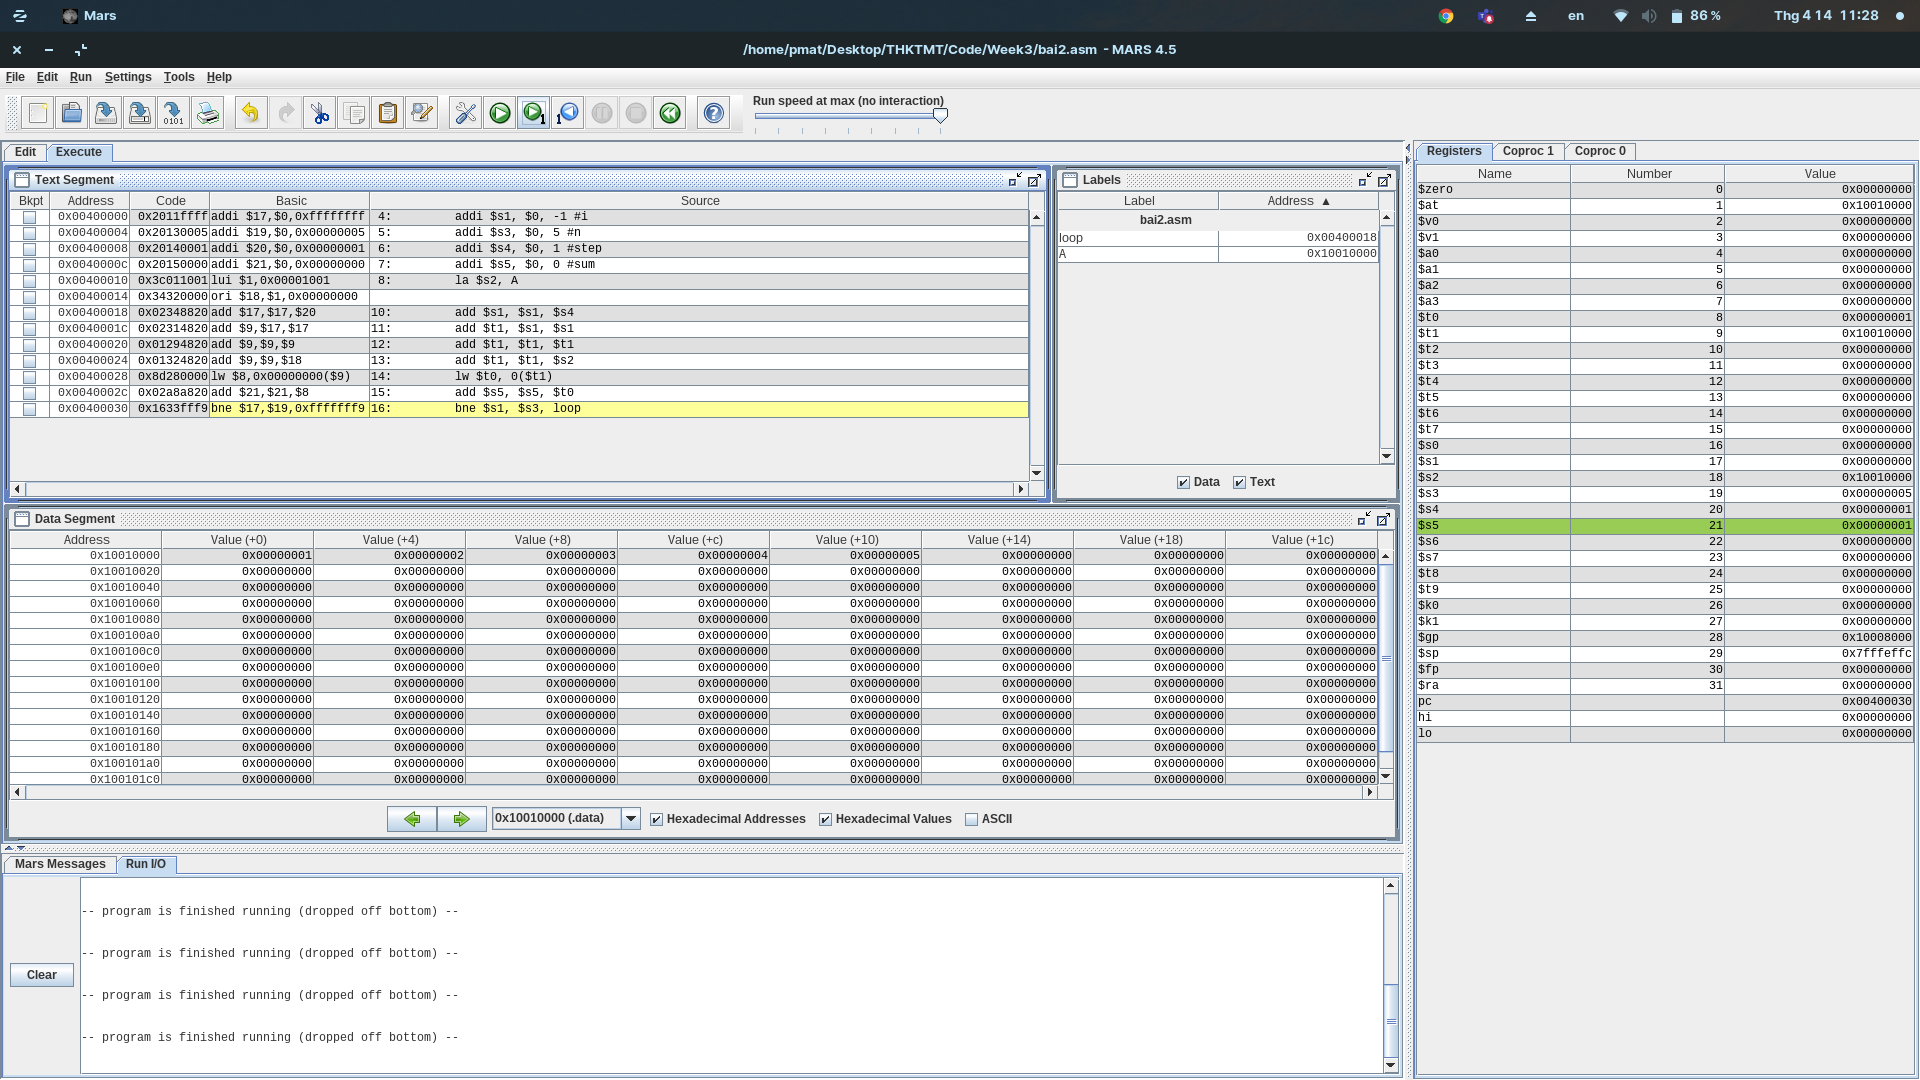
\includegraphics[width=0.7\textwidth]{ass2/s11.png}}}
	\caption*{Step 4: Cộng vào \$s5 (sum) giá trị hiện thời của mảng}
	\label{fig:2s4}
\end{figure}
\begin{figure}[!h]
	\centerline{\fbox{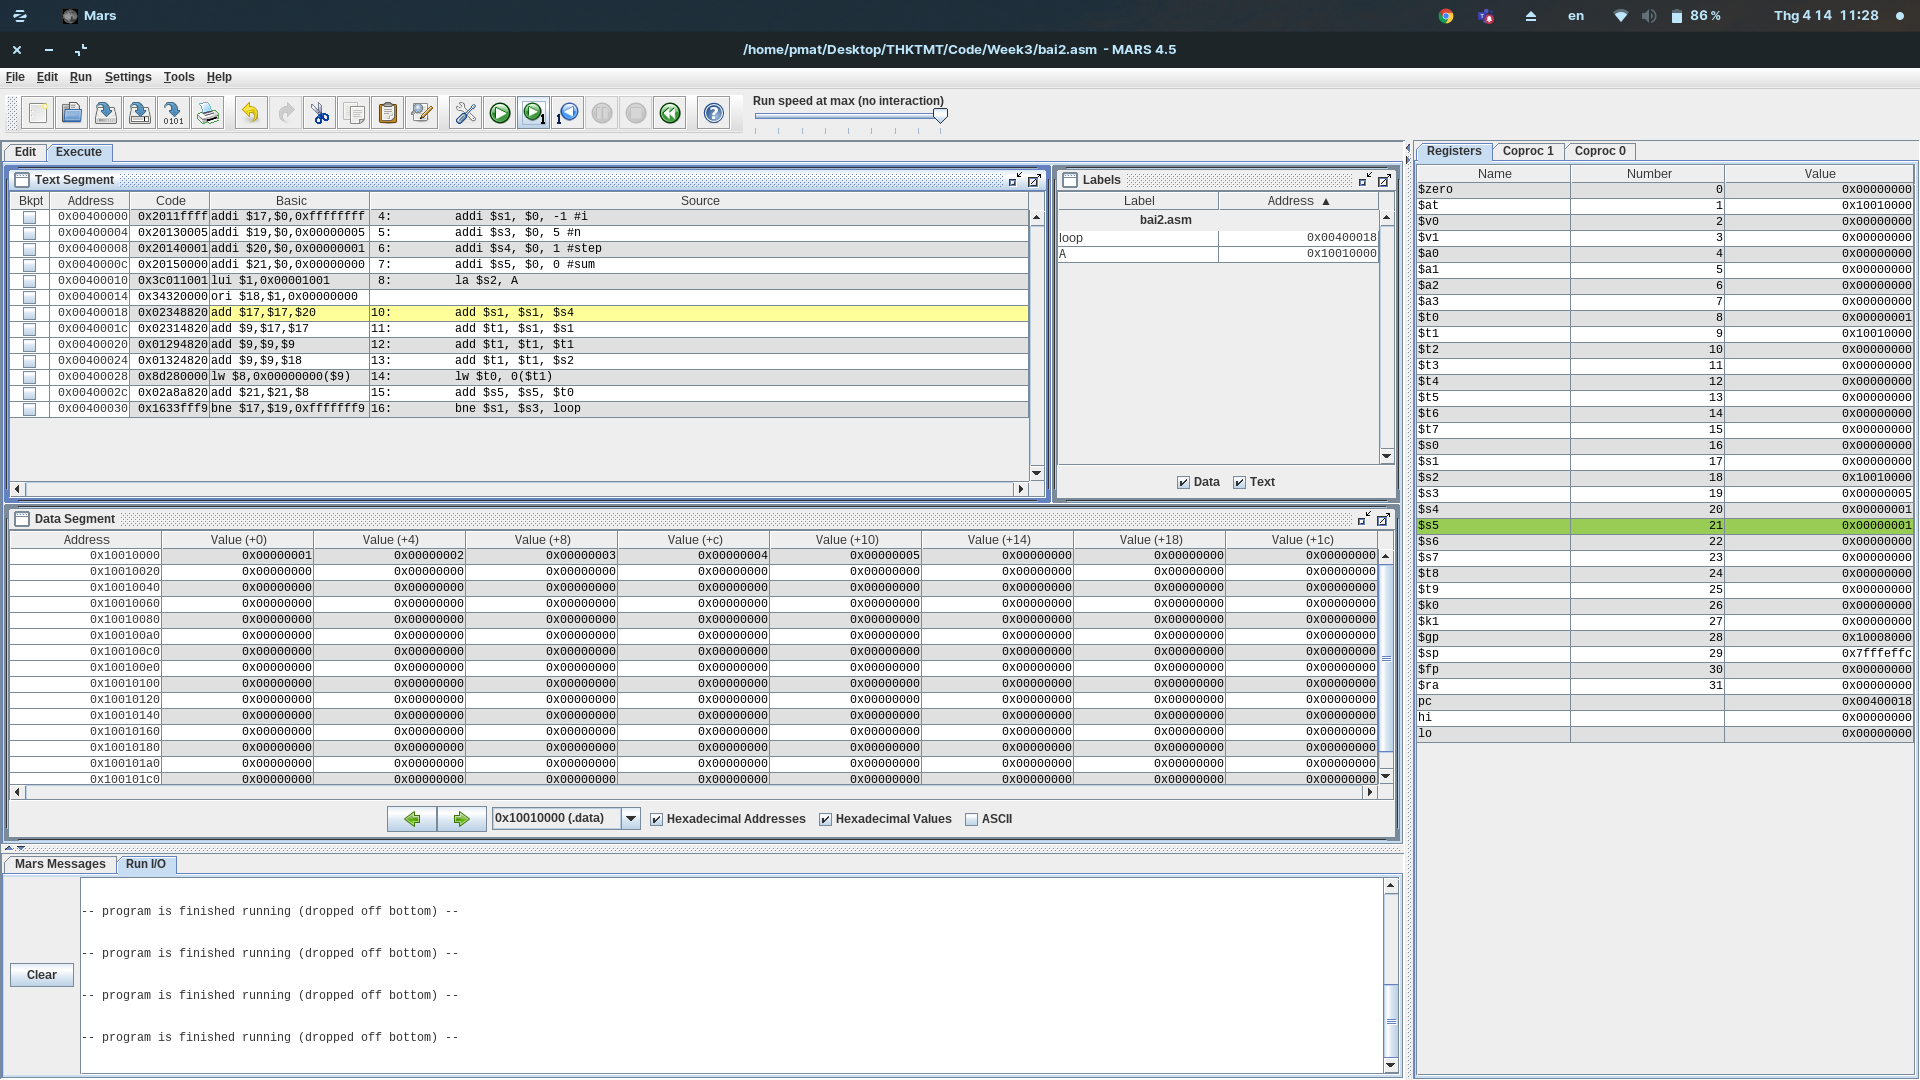
\includegraphics[width=0.7\textwidth]{ass2/s12.png}}}
	\caption*{Step 5: i != n, tiếp tục nhảy đến loop}
	\label{fig:2s5}
\end{figure}
\begin{figure}[!h]
	\centerline{\fbox{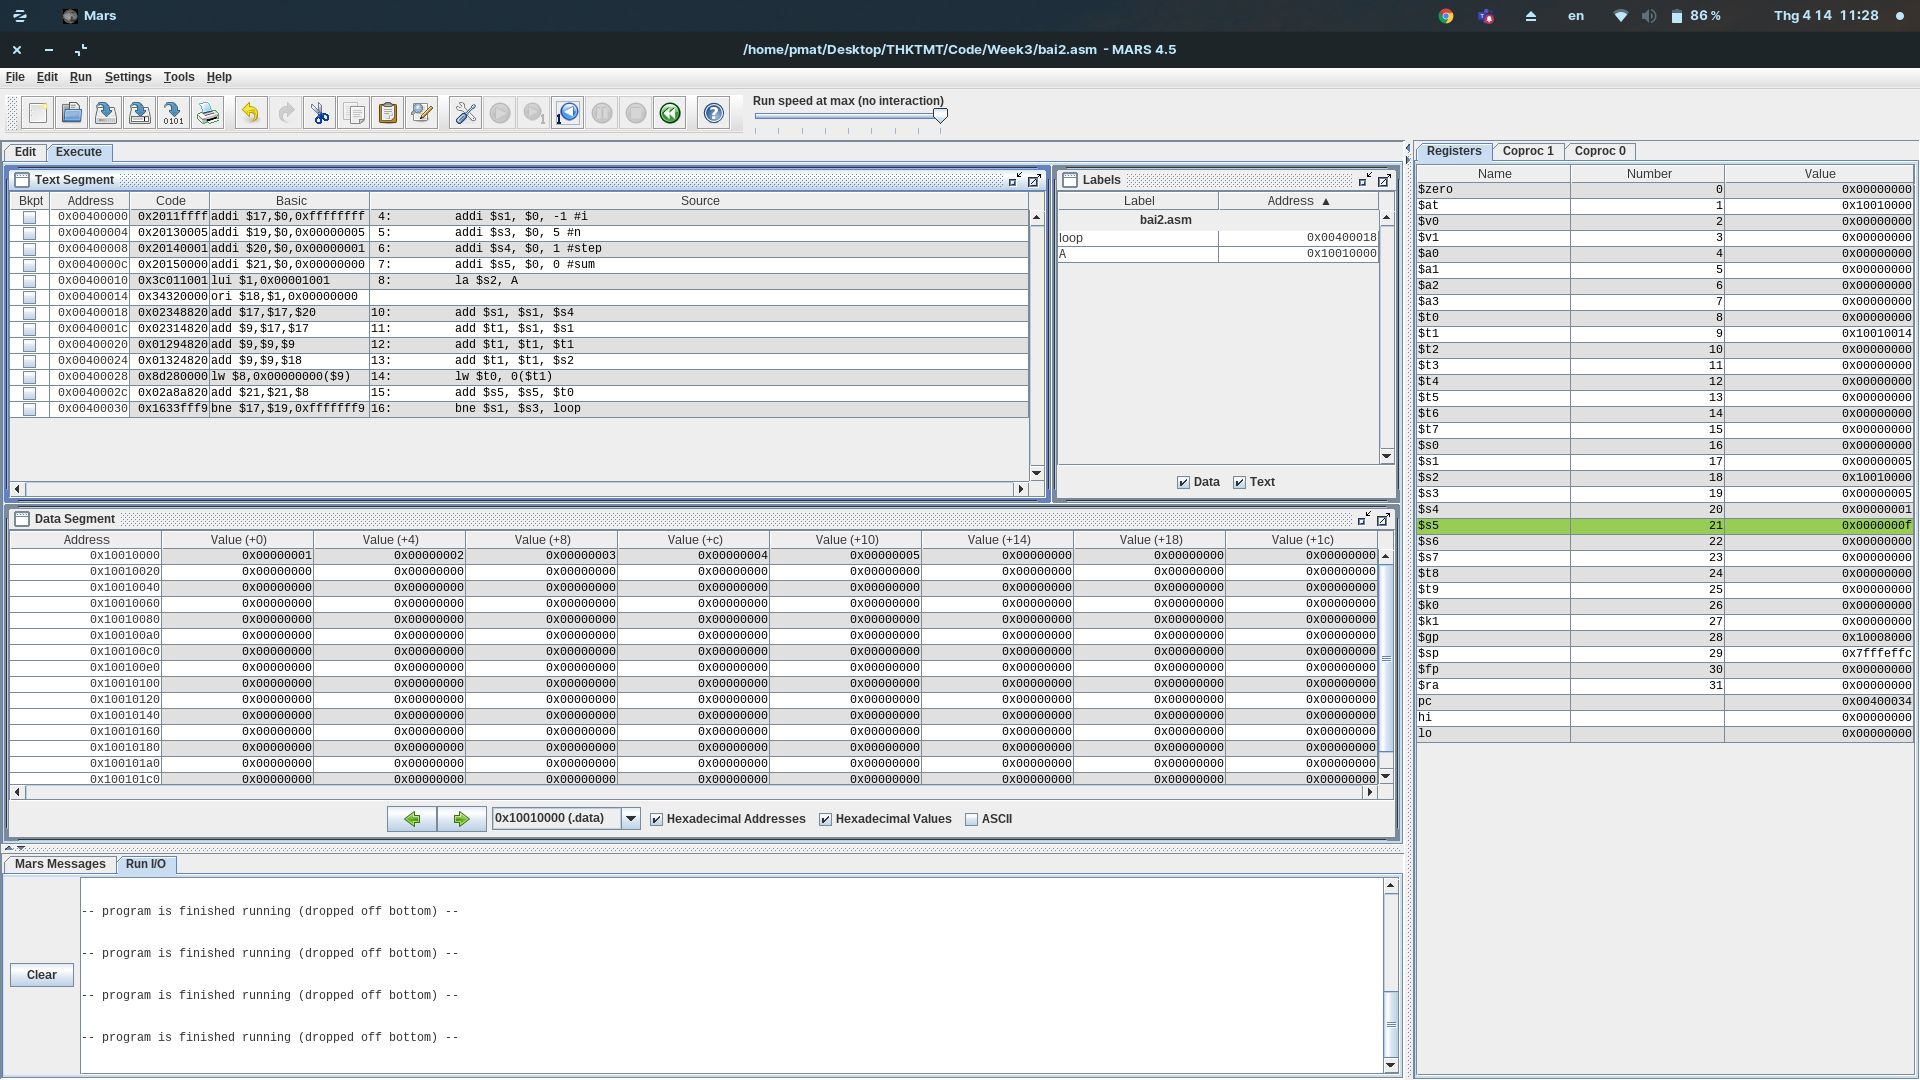
\includegraphics[width=0.7\textwidth]{ass2/s13.png}}}
	\caption*{Step 6: qua n vòng lặp, tổng của mảng là 0xf = 15 = 1+2+3+4+5}
	\label{fig:2s6}
\end{figure}
\clearpage
\newpage
\section{Assignment 3}
\begin{figure}[!h]
	\centerline{\fbox{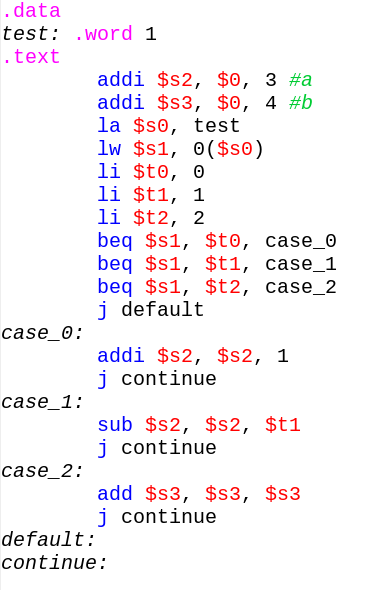
\includegraphics[width=0.7\textwidth]{ass3/ass3.png}}}
	\caption{Code của Assignment 3}
	\label{fig:ass3}
\end{figure}
\begin{figure}[!h]
	\centerline{\fbox{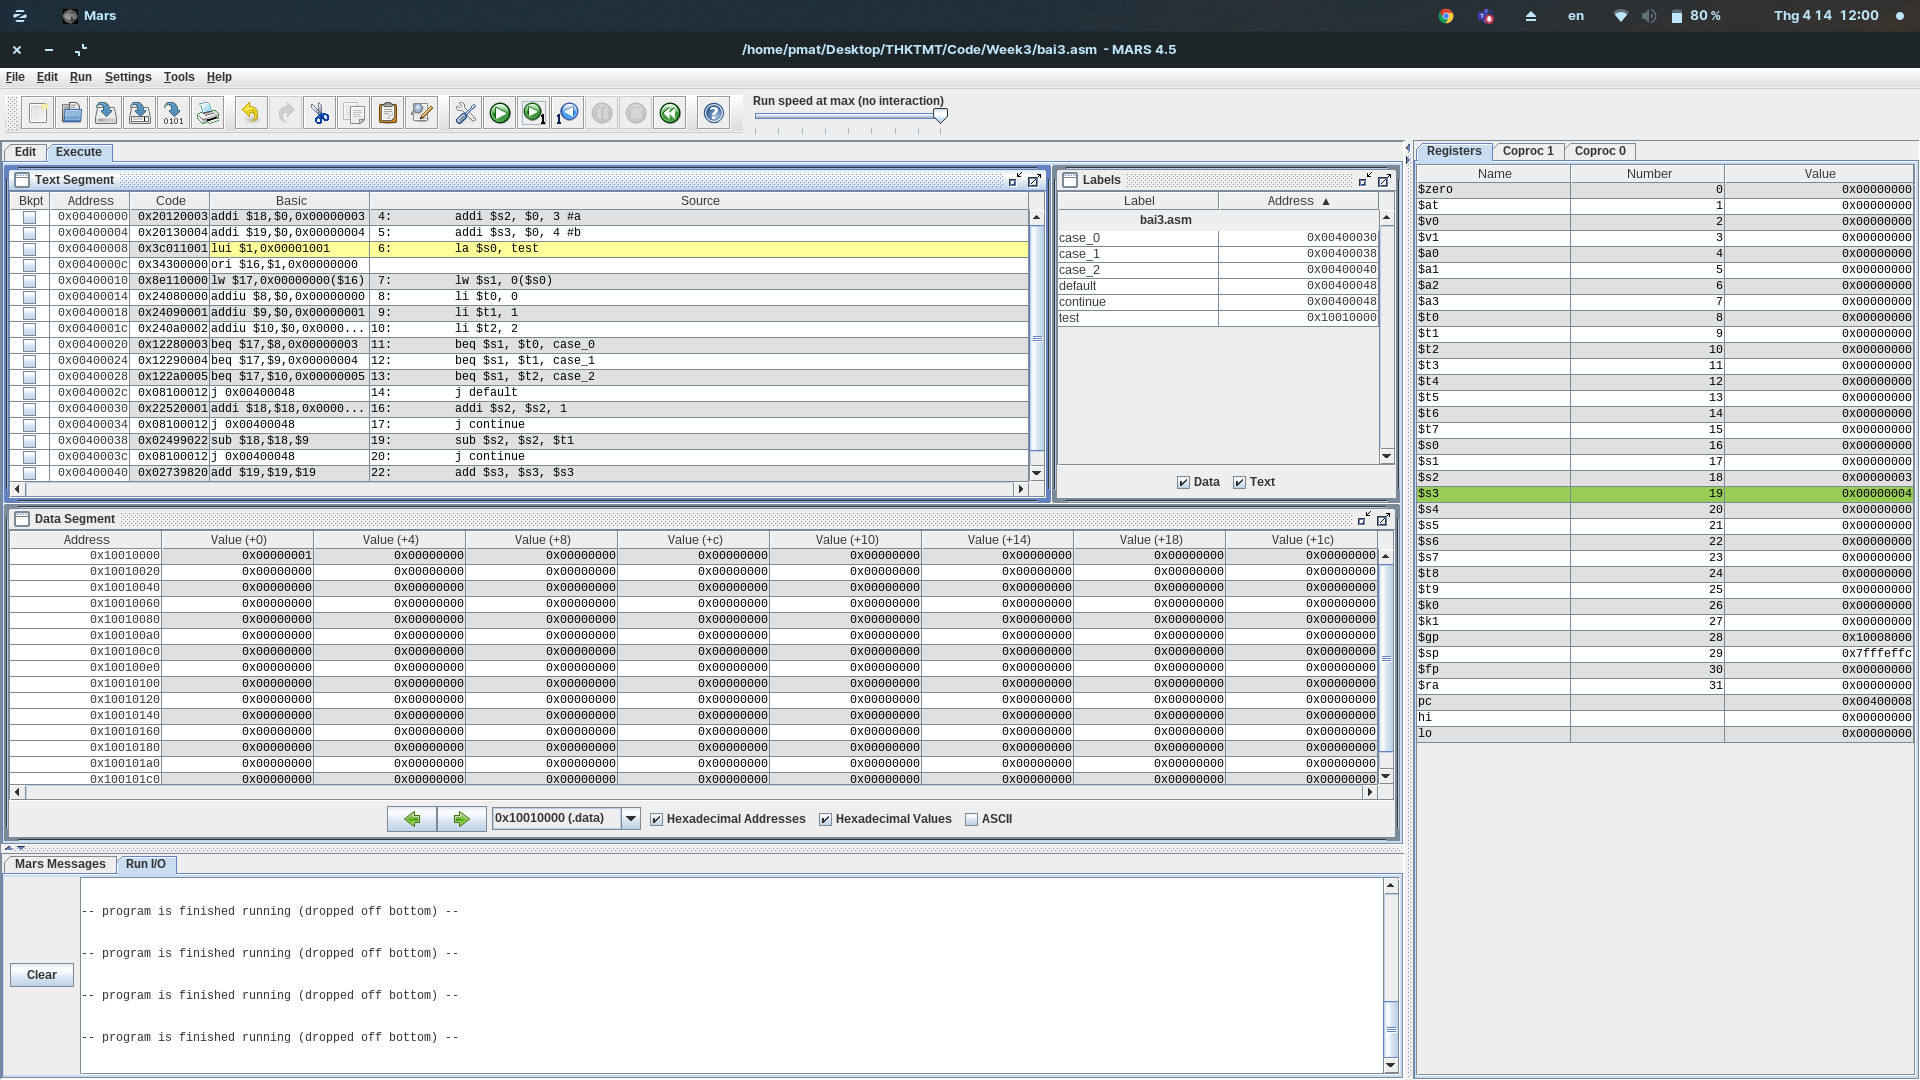
\includegraphics[width=0.7\textwidth]{ass3/s1.png}}}
	\caption*{Step 1: Gán giá trị thanh ghi lần lượt \$s2 = 3, \$s3 = 4}
	\label{fig:3s1}
\end{figure}
\begin{figure}[!h]
	\centerline{\fbox{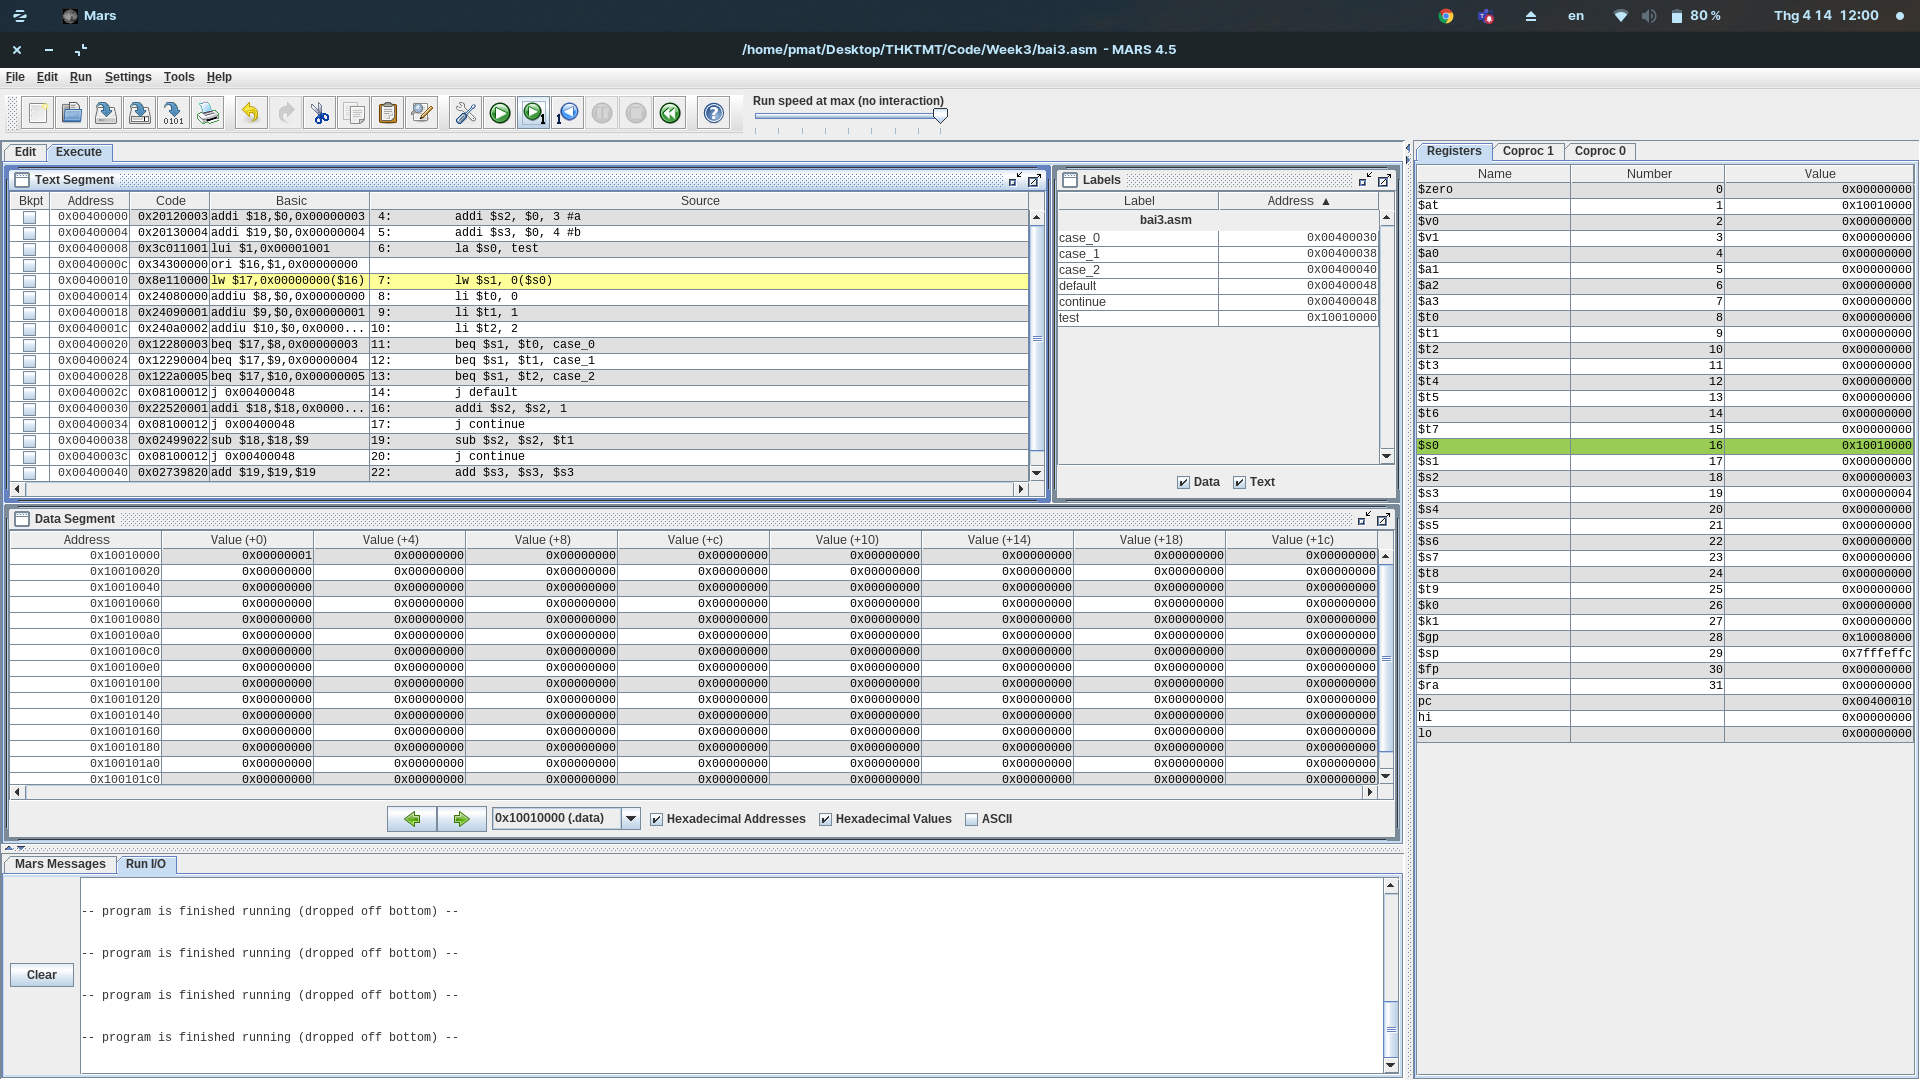
\includegraphics[width=0.7\textwidth]{ass3/s2.png}}}
	\caption*{Step 2: Load địa chỉ test vào \$s0}
	\label{fig:3s2}
\end{figure}
\begin{figure}[!h]
	\centerline{\fbox{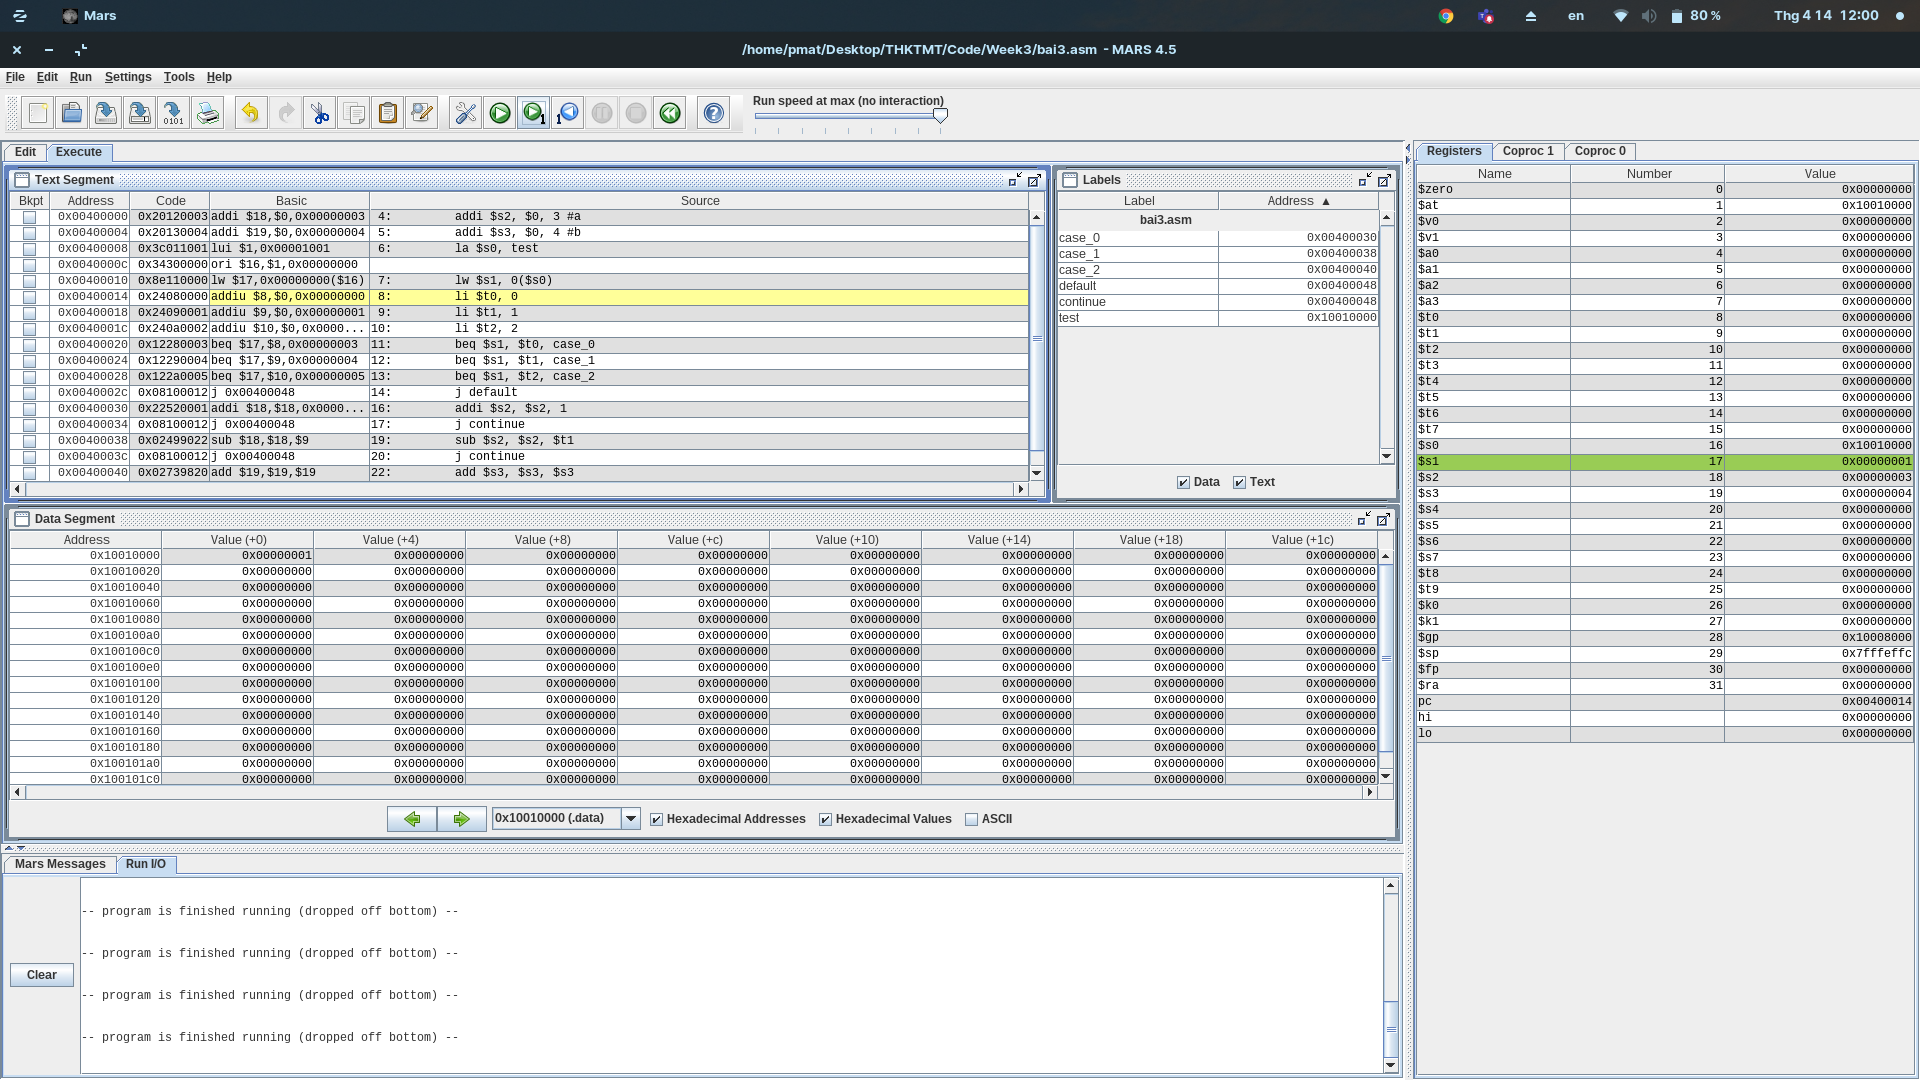
\includegraphics[width=0.7\textwidth]{ass3/s3.png}}}
	\caption*{Step 3: Lấy giá trị của \$s1 cho vào \$s0}
	\label{fig:3s3}
\end{figure}
\begin{figure}[!h]
	\centerline{\fbox{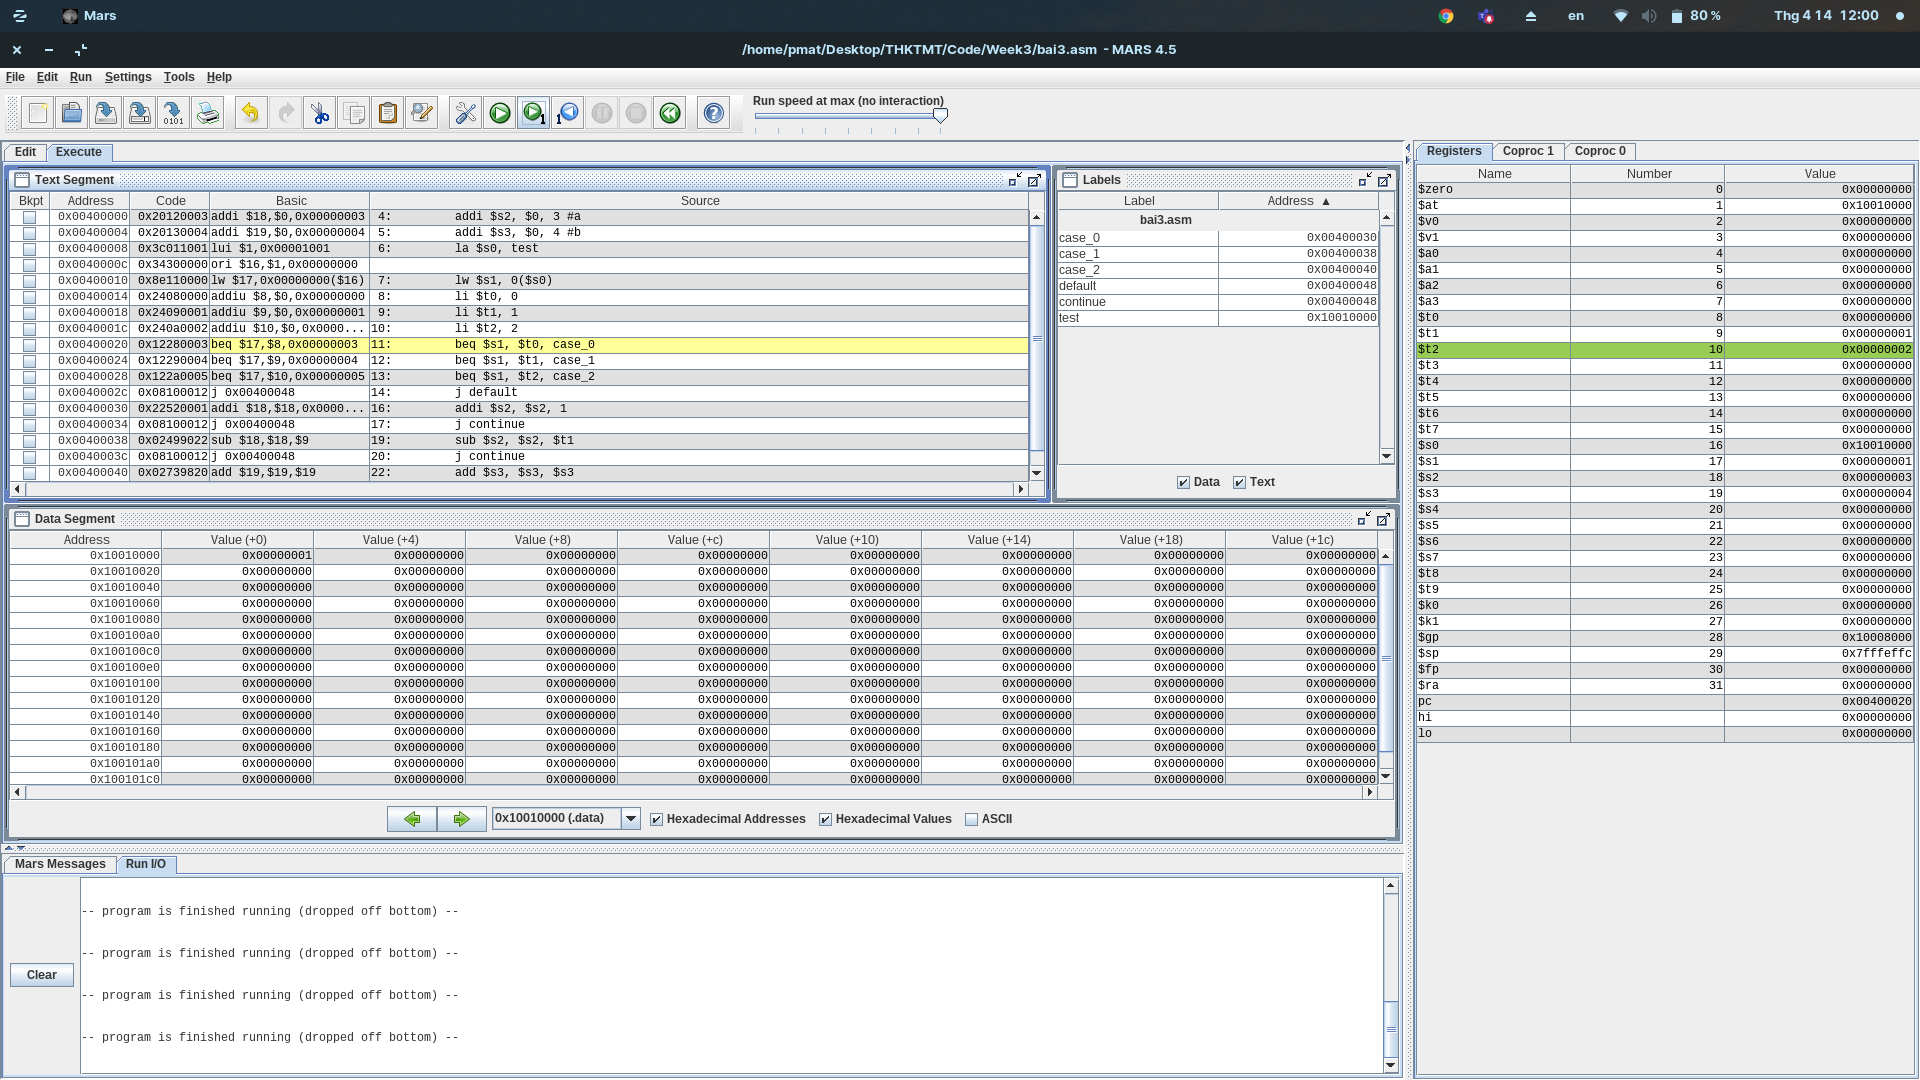
\includegraphics[width=0.7\textwidth]{ass3/s4.png}}}
	\caption*{Step 4: Gán tạm thời \$t0 = 0, \$t1 = 1, \$ t2 = 2}
	\label{fig:3s4}
\end{figure}
\begin{figure}[!h]
	\centerline{\fbox{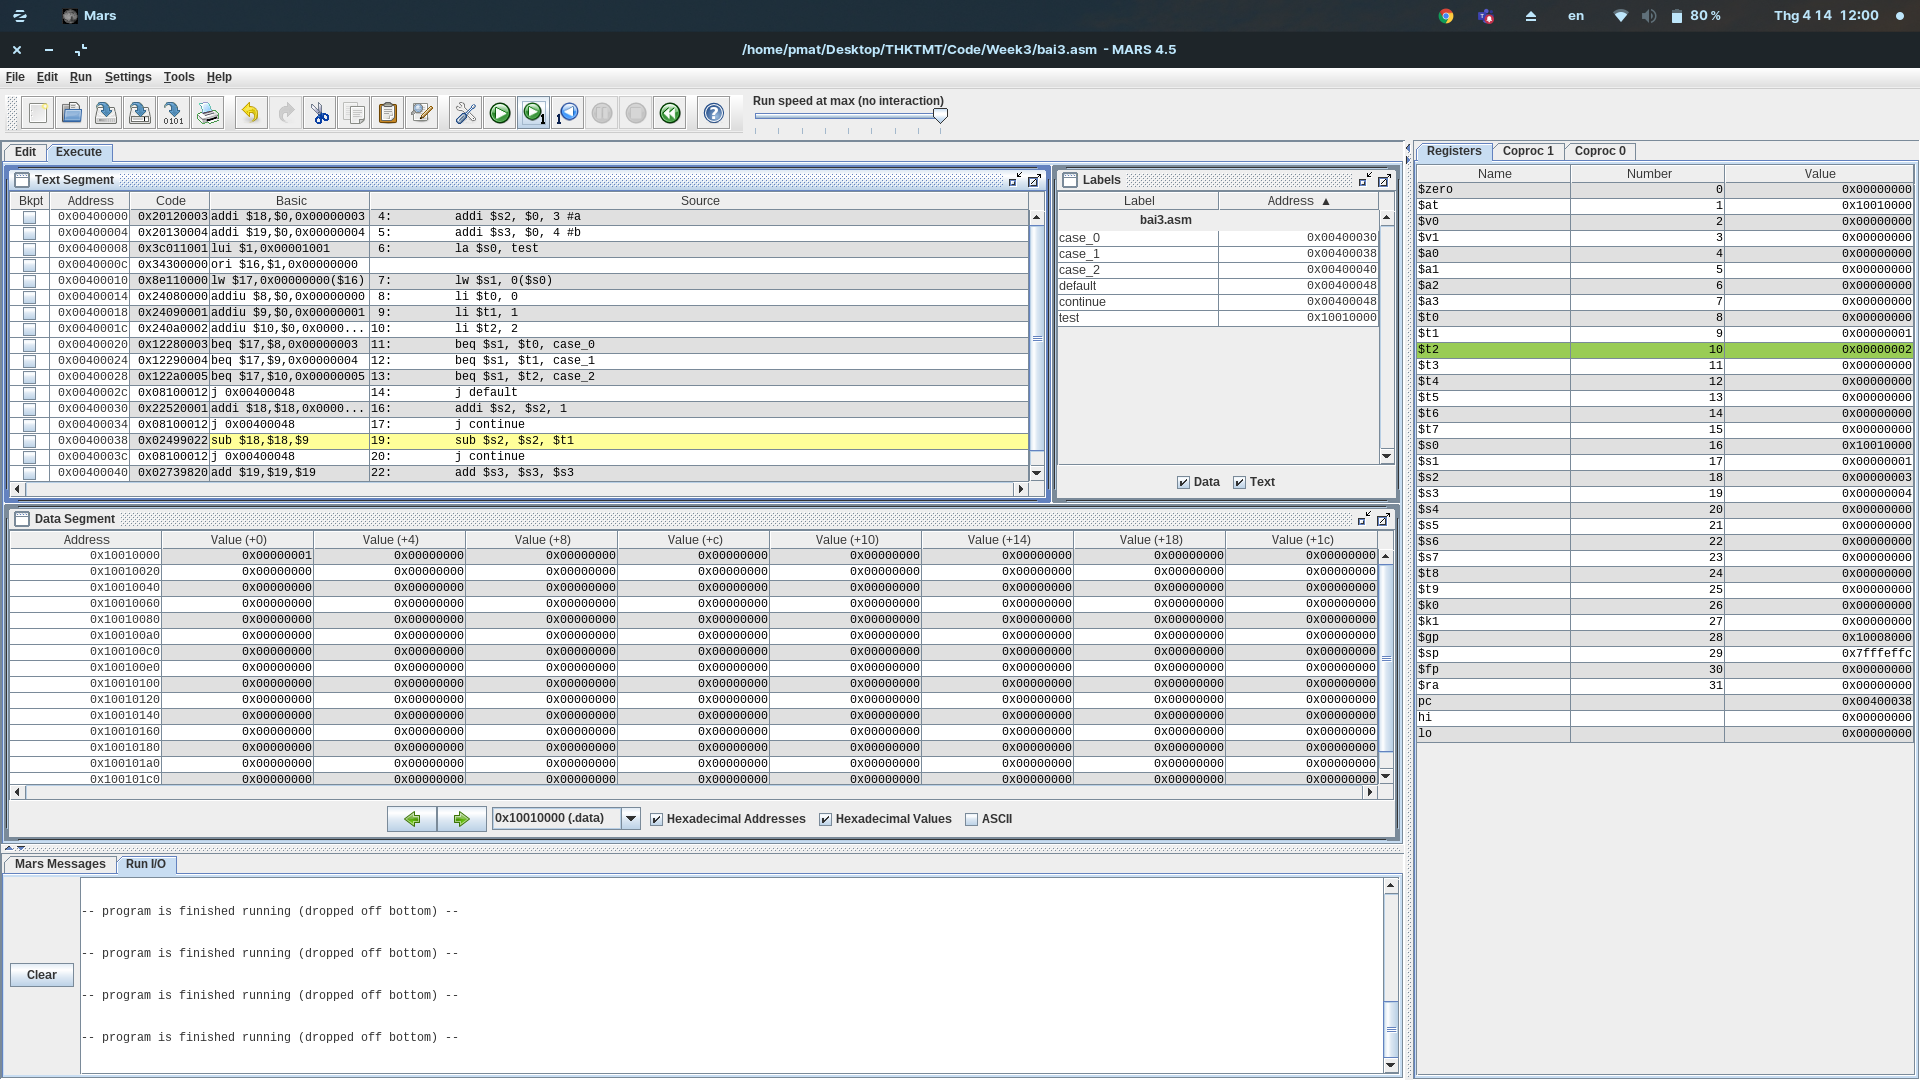
\includegraphics[width=0.7\textwidth]{ass3/s5.png}}}
	\caption*{Step 5: So sánh giá trị \$s1 với \$t0, \$t1, \$t2 để nhảy đến case tương ứng}
	\label{fig:3s5}
\end{figure}
\begin{figure}[!h]
	\centerline{\fbox{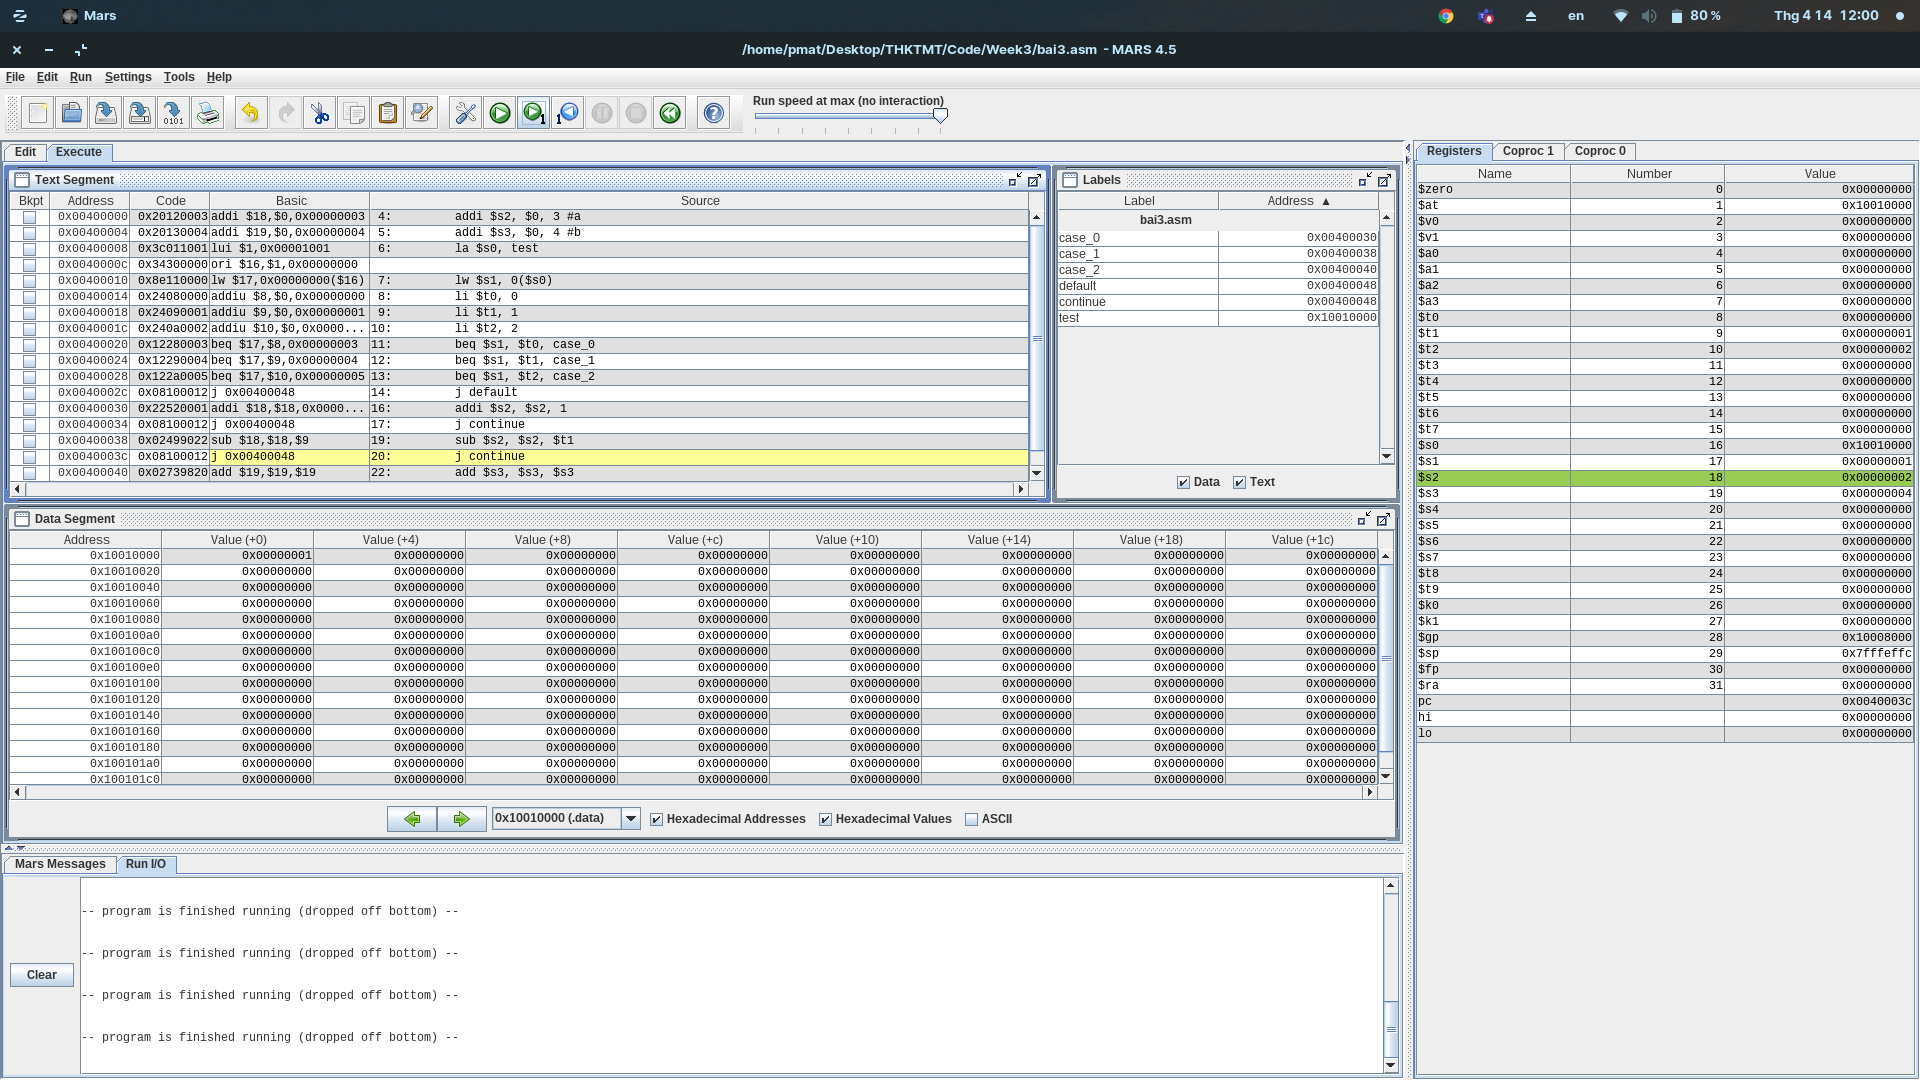
\includegraphics[width=0.7\textwidth]{ass3/s6.png}}}
	\caption*{Step 6: do \$s1 = \$t1 = 1, nhảy đến case 1, thực hiện \$s2 = \$s2 - \$t1 = \\ 3 - 1 = 2}
	\label{fig:3s6}
\end{figure}
\clearpage
\newpage
\begin{figure}[!h]
	\centerline{\fbox{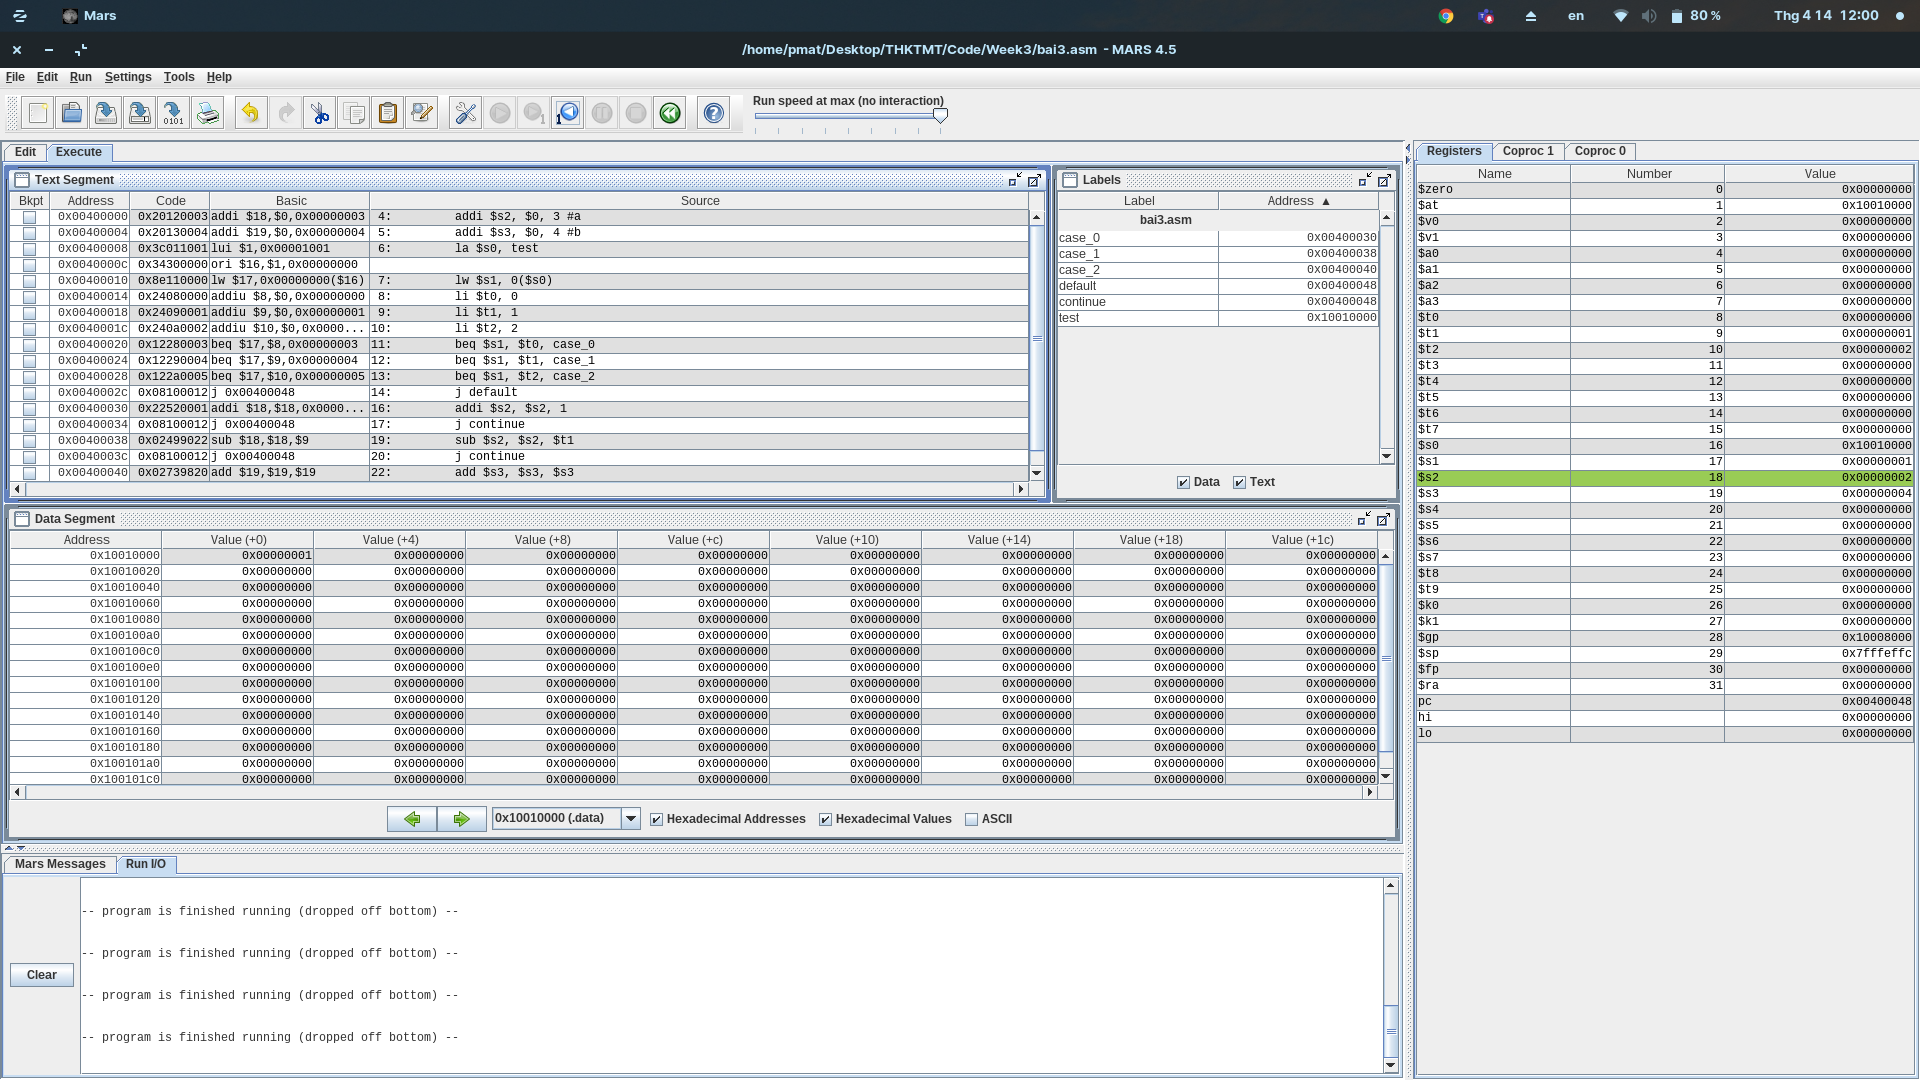
\includegraphics[width=0.7\textwidth]{ass3/s7.png}}}
	\caption*{Step 7: Thoát chương trình}
	\label{fig:3s7}
\end{figure}
\noindent 
Tương tự, khi test = 0, chương trình thực hiện case 0, \$s2 từ 3 tăng lên 4 qua biểu thức addi \$s2, \$s2, 1.
Khi test = 2, chương trình thực hiện case 2, \$s3 từ 4 tăng lên 8 qua biểu thức add \$s3, \$s3, \$s3.
\clearpage
\newpage
\section{Assignment 4}
\subsection{Assignment 4a}
\begin{figure}[!h]
	\centerline{\fbox{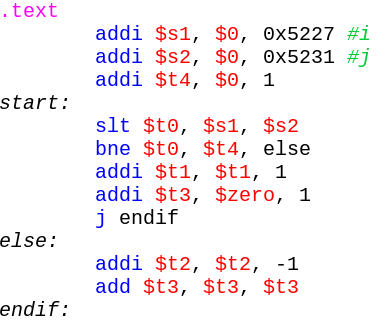
\includegraphics[width=0.7\textwidth]{ass4/ass4a.png}}}
	\caption{Code của Assignment 4a}
	\label{fig:ass4}
\end{figure}
\noindent
Thay đổi dòng 5 và dòng 6, so sánh \$s1 (i) và \$s2(j) để trả về \$t0 sau đó thực hiện so sánh với \$t4 có giá trị bằng 1. Nếu i < j, \$t0 = 1, thực hiện dòng lệnh dưới không nhảy đến else, ngược lại, nhảy đến else và thực hiện lệnh. \\
\clearpage
\newpage
\subsection{Assignment 4b}
\begin{figure}[!h]
	\centerline{\fbox{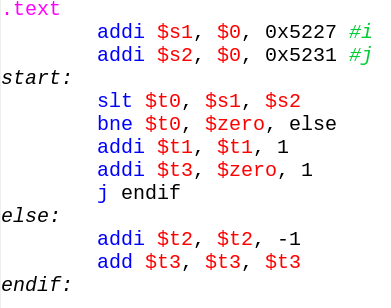
\includegraphics[width=0.7\textwidth]{ass4/ass4b.png}}}
	\caption{Code của Assignment 4b}
	\label{fig:ass4b}
\end{figure}
\noindent
Đảo chỗ \$s1 \$s2 ở dòng 5 so với assignment 1. \\ 
\clearpage
\newpage
\subsection{Assignment 4c}
\begin{figure}[!h]
	\centerline{\fbox{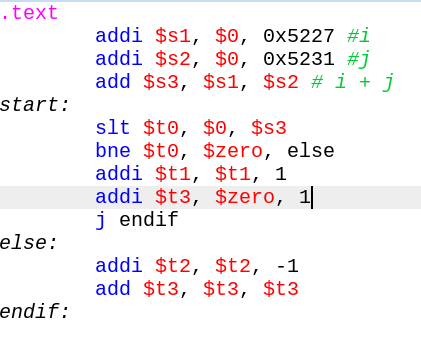
\includegraphics[width=0.7\textwidth]{ass4/ass4c.png}}}
	\caption{Code của Assignment 4c}
	\label{fig:ass4c}
\end{figure}
\noindent
Gán giá trị \$s3 là tổng \$s1 và \$s2, thực hiện so sánh với 0. \\ 
\clearpage
\newpage
\subsection{Assignment 4d}
\begin{figure}[!h]
	\centerline{\fbox{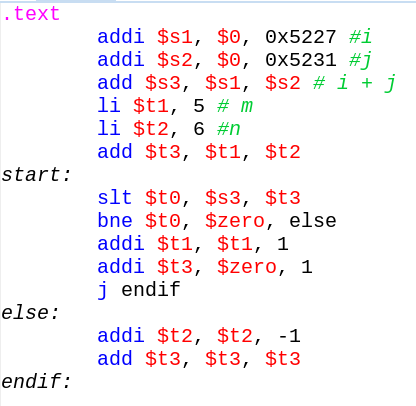
\includegraphics[width=0.7\textwidth]{ass4/ass4d.png}}}
	\caption{Code của Assignment 4d}
	\label{fig:ass4d}
\end{figure}
\noindent
Gán giá trị \$s3 là tổng \$s1 và \$s2. Khởi tạo m là 5, n là 6. Gán giá trị \$t3 là m + n. Sau đó thực hiện so sánh \$s3 và \$t3. \\
\clearpage
\newpage
\section{Assignment 5}
\subsection{Assignment 5a}
\begin{figure}[!h]
	\centerline{\fbox{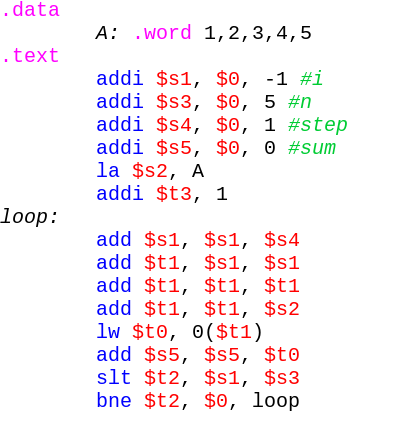
\includegraphics[width=0.7\textwidth]{ass5/ass5a.png}}}
	\caption{Code của Assignment 5a}
	\label{fig:ass5a}
\end{figure}
\noindent
So sánh \$s1 (i) và \$s2 (n). Nếu i < n, \$t2 trả về 1, khác \$0 nên tiếp tục vòng lặp. Ngược lại dừng vòng lặp. \\ 
\clearpage
\newpage
\subsection{Assignment 5b}
\begin{figure}[!h]
	\centerline{\fbox{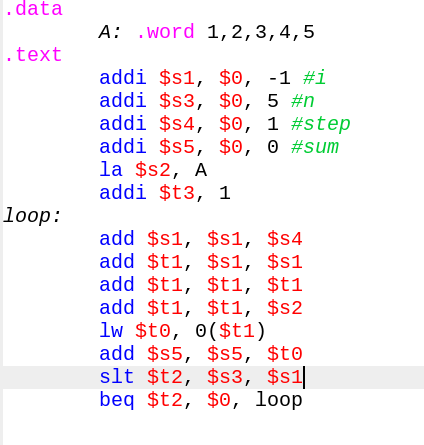
\includegraphics[width=0.7\textwidth]{ass5/ass5b.png}}}
	\caption{Code của Assignment 5b}
	\label{fig:ass5b}
\end{figure}
\noindent
So sánh \$s1 (i) và \$s2 (n). Nếu n < i, \$t2 trả về 1, ngược lại \$t2 trả về 0. So sánh \$t2 và 0, nếu bằng nhau thực hiện loop, ngược lại dừng vòng lặp
\clearpage
\newpage
\subsection{Assignment 5c}
\begin{figure}[!h]
	\centerline{\fbox{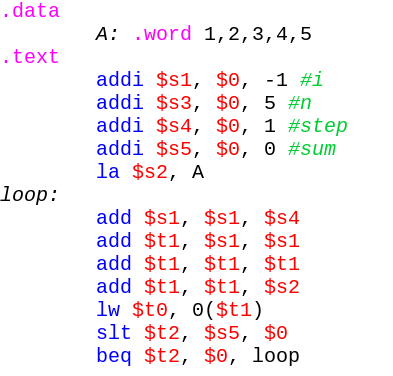
\includegraphics[width=0.7\textwidth]{ass5/ass5c.png}}}
	\caption{Code của Assignment 5c}
	\label{fig:ass5c}
\end{figure}
\noindent
So sánh 0 và sum. Nếu sum < 0, \$t2 trả về 1 != 0 dừng vòng lặp. Ngược lại tiếp tục vòng lặp. \\
\clearpage
\newpage
\subsection{Assignment 5d}
\begin{figure}[!h]
	\centerline{\fbox{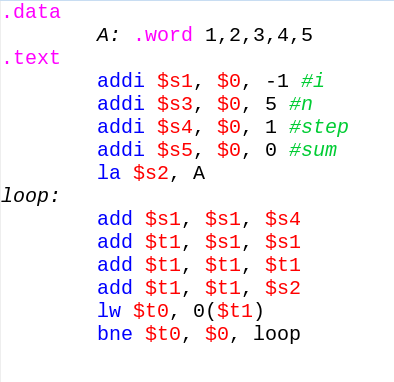
\includegraphics[width=0.7\textwidth]{ass5/ass5d.png}}}
	\caption{Code của Assignment 5d}
	\label{fig:ass5d}
\end{figure}
\noindent
So sánh \$t0 là giá trị trỏ đến mạng tại ngay lúc đó. Nếu \$t0 khác 0 tiếp tục vòng lặp, ngược lại dừng vòng lặp. \\
\clearpage
\newpage
\section{Assignment 6}
\begin{figure}[!h]
	\centerline{\fbox{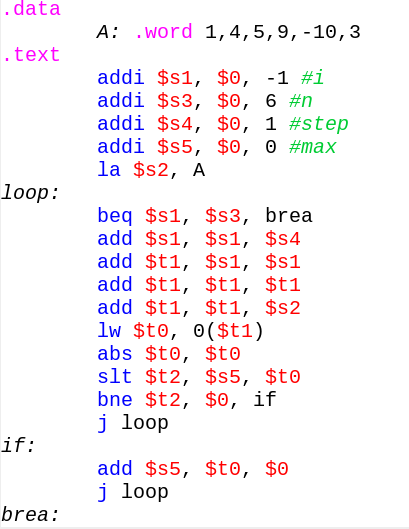
\includegraphics[width=0.7\textwidth]{ass6/ass6.png}}}
	\caption{Code của Assignment 6}
	\label{fig:ass6}
\end{figure}
\noindent
Giải thích thuật toán: 
\begin{itemize}
	\item Tại mỗi vòng lặp, kiểm tra xem i != n không, nếu không rời vòng lặp
	\item Tại dòng 16, lấy trị tuyệt đối của giá trị hiện thời của mảng
	\item Nếu tổng \$s5 < giá trị hiện thời \$t0  thì tiến hành gán \$s5 = \$t0. Nếu không tiếp tục vòng lặp
\end{itemize}
\begin{figure}[!h]
	\centerline{\fbox{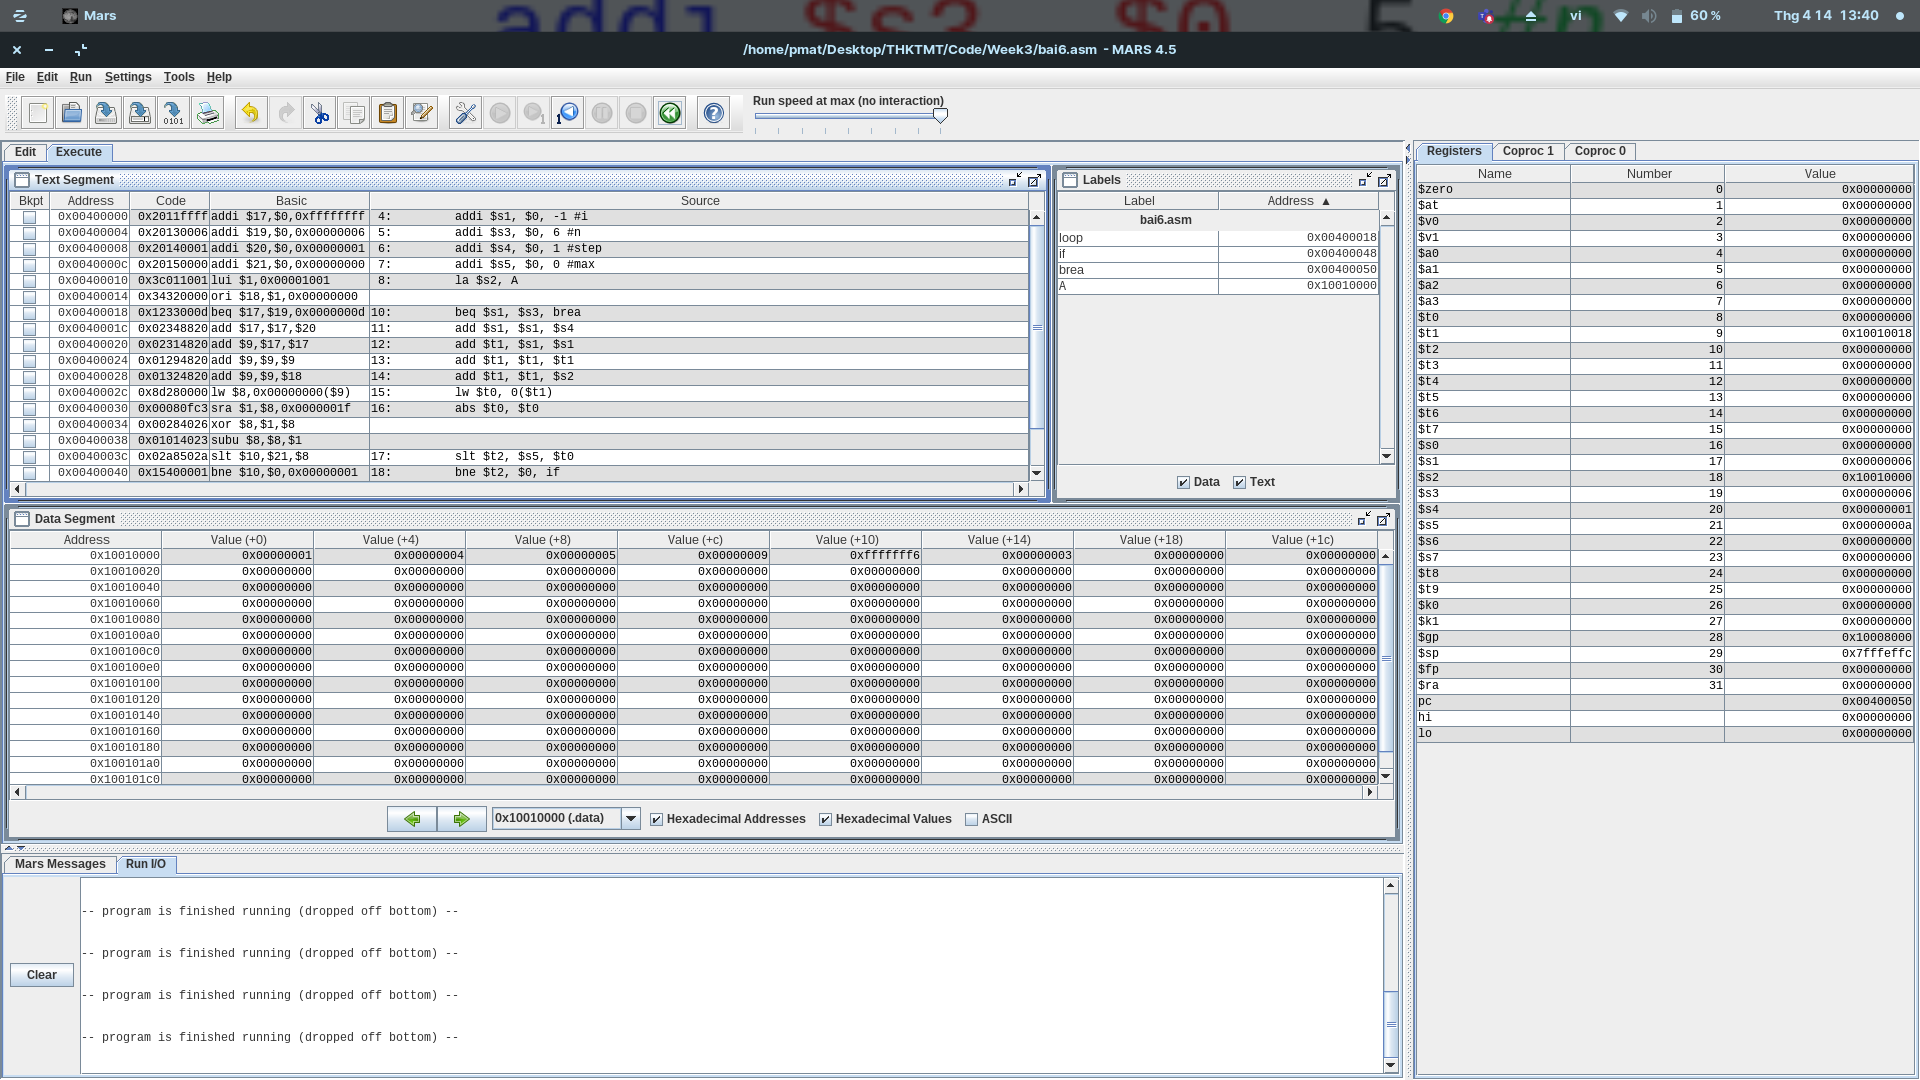
\includegraphics[width=1\textwidth]{ass6/result.png}}}
	\caption{Kết quả tại thanh ghi \$s5}
	\label{fig:ass6a}
\end{figure}
\end{document}